%% uctest.tex 11/3/94
%% Copyright (C) 1988-2004 Daniel Gildea, BBF, Ethan Munson.
%
% This work may be distributed and/or modified under the
% conditions of the LaTeX Project Public License, either version 1.3
% of this license or (at your option) any later version.
% The latest version of this license is in
%   http://www.latex-project.org/lppl.txt
% and version 1.3 or later is part of all distributions of LaTeX
% version 2003/12/01 or later.
%
% This work has the LPPL maintenance status "maintained".
% 
% The Current Maintainer of this work is Daniel Gildea.

\documentclass[12pt]{ucthesis}
\def\dsp{\def\baselinestretch{2.0}\large\normalsize}
\dsp

%%BIBLIOGRAPHY- This uses biber/biblatex to generate bibliographies according to the
%%Unified Style Sheet for Linguistics
\usepackage[main=american, german]{babel}% Recommended
\usepackage{csquotes}% Recommended
\usepackage[backend=biber,
        style=unified,
        maxcitenames=3,
        maxbibnames=99,
        natbib,
        url=false]{biblatex}
\addbibresource{Dissertation.bib}
\setcounter{biburlnumpenalty}{100}  % allow URL breaks at numbers
% \setcounter{biburlucpenalty}{100}   % allow URL breaks at uppercase letters
% \setcounter{biburllcpenalty}{100}   % allow URL breaks at lowercase letters

%%TYPOLOGY  
\usepackage{tipa} %International Phonetic Alphabet
\usepackage[colorlinks,allcolors={black},urlcolor={blue}]{hyperref} %allows for hyperlinks and pdf bookmarks 
\usepackage{graphicx}	%Inserting graphics, pictures, images 		
\usepackage{fontspec} %Selection of fonts must be ran in XeLaTeX or LuaLateX
\usepackage{amssymb} %Math symbols
\usepackage{amsmath} % Mathematical enhancements for LaTeX
\usepackage{multicol} %Multicolumn text
\usepackage{enumitem} %Allows for continuous numbering of lists over examples, etc.
\usepackage{multirow} %Useful for combining cells in tablesbrew 
% \usepackage[colorlinks,allcolors={black},urlcolor={blue}]{hyperref} %allows for hyperlinks and pdf bookmarks
% \usepackage{url} %allows for urls
% \def\UrlBreaks{\do\/\do-} %allows for urls to be broken up
% \usepackage[normalem]{ulem} %strike out text. Handy for syntax
% \usepackage{tcolorbox}
% \usepackage{todonotes} % Creates todo marginalia

%%FONTS
\setmainfont{Libertinus Serif}
\setsansfont{Libertinus Sans}
% \setmonofont[Scale=MatchLowercase]{Libertinus Mono}

%%PACKAGES FOR LINGUISTICS
%\usepackage{OTtablx} %Generating tableaux with using TIPA
% \usepackage[noipa]{OTtablx} % Use this one generating tableaux without using TIPA
%\usepackage[notipa]{ot-tableau} % Another tableau drawing packing use for posters.
% \usepackage{linguex} % Linguistic examples
% \usepackage{langsci-linguex} % Linguistic examples
\usepackage{langsci-gb4e} % Language Science Press' modification of gb4e
% \usepackage{langsci-avm} % Language Science Press' AVM package
% \usepackage{tikz} % Drawing Hasse diagrams
% \usepackage{pst-asr} % Drawing autosegmental features
% \usepackage{pstricks} % required for pst-asr, OTtablx, pst-jtree.
% \usepackage{pst-jtree} 	% Syntax tree draawing software
% \usepackage{tikz-qtree}	% Another syntax tree drawing software. Uses bracket notation.
% \usepackage[linguistics]{forest}	% Another syntax tree drawing software. Uses bracket notation.
% \usepackage{ling-macros} % Various linguistic macros. Does not work with linguex.
% \usepackage{covington} % Another linguistic examples package.
\usepackage{leipzig} %	Offers support for Leipzig Glossing Rules

%%LEIPZIG GLOSSING FOR ZAPOTEC
\newleipzig{el}{el}{elder} % Elder pronouns
\newleipzig{hu}{hu}{human} % Human pronouns
\newleipzig{an}{an}{animate} % Animate pronouns
\newleipzig{in}{in}{inanimate} % Inanimate pronouns
\newleipzig{pot}{pot}{potential} % Potential Aspect
\newleipzig{cont}{cont}{continuative} % Continuative Aspect
\newleipzig{stat}{stat}{stative} % Stative Aspect
\newleipzig{and}{and}{andative} % Andative Aspect
\newleipzig{ven}{ven}{venative} % Venative Aspect
% \newleipzig{res}{res}{restitutive} % Restitutive Aspect
\newleipzig{rep}{rep}{repetitive} % Repetitive Aspect


\begin{document}

% Declarations for Front Matter

\title{Voice Quality and Tone at the phonetics and phonology interface}
\author{Mykel L. Brinkerhoff}
\degreeyear{2025}
\degreemonth{June}
\degree{DOCTOR OF PHILOSOPHY}
\chair{Professor Grant McGuire}
\committeememberone{Professor Jaye Padgett}
\committeemembertwo{Professor Ryan Bennett}
\committeememberthree{Professor Marc Garellek}
\numberofmembers{4} %% (including chair) possible: 3, 4, 5, 6
\deanlineone{Peter Biehl}
\deanlinetwo{Vice Provost and Dean of Graduate Studies}
\deanlinethree{}
\field{Linguistics}
\campus{Santa Cruz}

\begin{frontmatter}

\maketitle
\copyrightpage

\tableofcontents
\listoffigures
\listoftables

\begin{abstract}
    This dissertation provides a detailed description and analysis of the SLZ voice quality system, a minority language spoken by about 1000 people in the municipality of Santiago Laxopa, and its interactions with the tonal system of the language. Standard assumptions about the interaction between tone and voice quality in Otomanguean languages proposed by \citet{silvermanLaryngealComplexityOtomanguean1997,silvermanPhasingRecoverability1997}, where nonmodal phonation is realized in only a portion of the vowel and tone is realized on a modal portion, do not fully hold in Santiago Laxopa Zapotec. Instead, speakers routinely produce nonmodal phonation throughout the entire vowel for breathy vowels. The only time phasing is observed is with the two types of creaky voice that occur in the language: rearticulated and checked. Rearticulated vowels have a period of creakiness in the middle of the vowel, whereas checked vowels have creakiness at the end. Although this creakiness is pronounced in distinct locations, non-modal phonation remains throughout the entire vowel. These results were confirmed through statistical modeling.

    ...

\end{abstract}
\begin{dedication}
\null\vfil
{\large
\begin{center}
Dedicated to my family,\\\vspace{12pt}
Betsy and Maelyn,\\\vspace{12pt}
I wouldn't be here without you.\\\vspace{12pt}
\end{center}}
\vfil\null
\end{dedication}
\begin{acknowledgements}
    When it comes to acknowledgements, there are so many words that could be said, but they often feel awkward and do not actually . There are many people who have helped me along the way, from my family to my friends, to my colleagues and mentors. I am grateful to all of them. 

    ... 
    
    % I would like to thank my advisor, Professor Grant McGuire, for his guidance and support throughout my time in graduate school. I would also like to thank my committee members, Professor Jaye Padgett, Professor Ryan Bennett, and Professor Marc Garellek, for their feedback and advice.

    % I would like to thank my family for their love and support. I would also like to thank my friends for their encouragement and understanding.

    % Finally, I would like to thank my wife, Betsy for their patience and understanding. I could not have done this without them.
\end{acknowledgements}



\end{frontmatter}

\chapter{Introduction}
%--------------------------------------------------------------------
%
% File: 2.SLZ.tex
% Author: Mykel Loren Brinkerhoff
% Description: Chapter on the Vowels and suprasegmentals in Santiago Laxopa Zapotec
%
%--------------------------------------------------------------------




\chapter{Vowels and suprasegmentals in Santiago Laxopa Zapotec} \label{ch:SLZ}

%-------------------------
\section{Introduction} \label{sec:SLZ-intro}
%-------------------------

Santiago Laxopa Zapotec (SLZ; \textit{Dilla'xhunh Laxup} [diʒaˀʐun lːaʂupʰ]) is a Northern Zapotec language spoken by approximately 1000 people in the municipality of Santiago Laxopa, Ixtlán,Oaxaca, Mexico and in diaspora communities throughout Mexico and the United States \citep{adlerAcousticsPhonationTypes2016,adlerDerivationVerbInitiality2018,foleyForbiddenCliticClusters2018,foleyExtendingPersonCaseConstraint2020}. 
According to \citet{smith-starkAlgunasIsoglosasZapotecas2007}, SLZ is part of the Cajonos Zapotec macro variety, which also includes Zoogocho Zapotec, Yatzachi Zapotec, Yalálag Zapotec, Tabaá Zapotec, Lachirioag Zapotec and several other varieties spoken in the Sierra Norte of Oaxaca, Mexico.

\begin{figure}[!h]
    \centering
    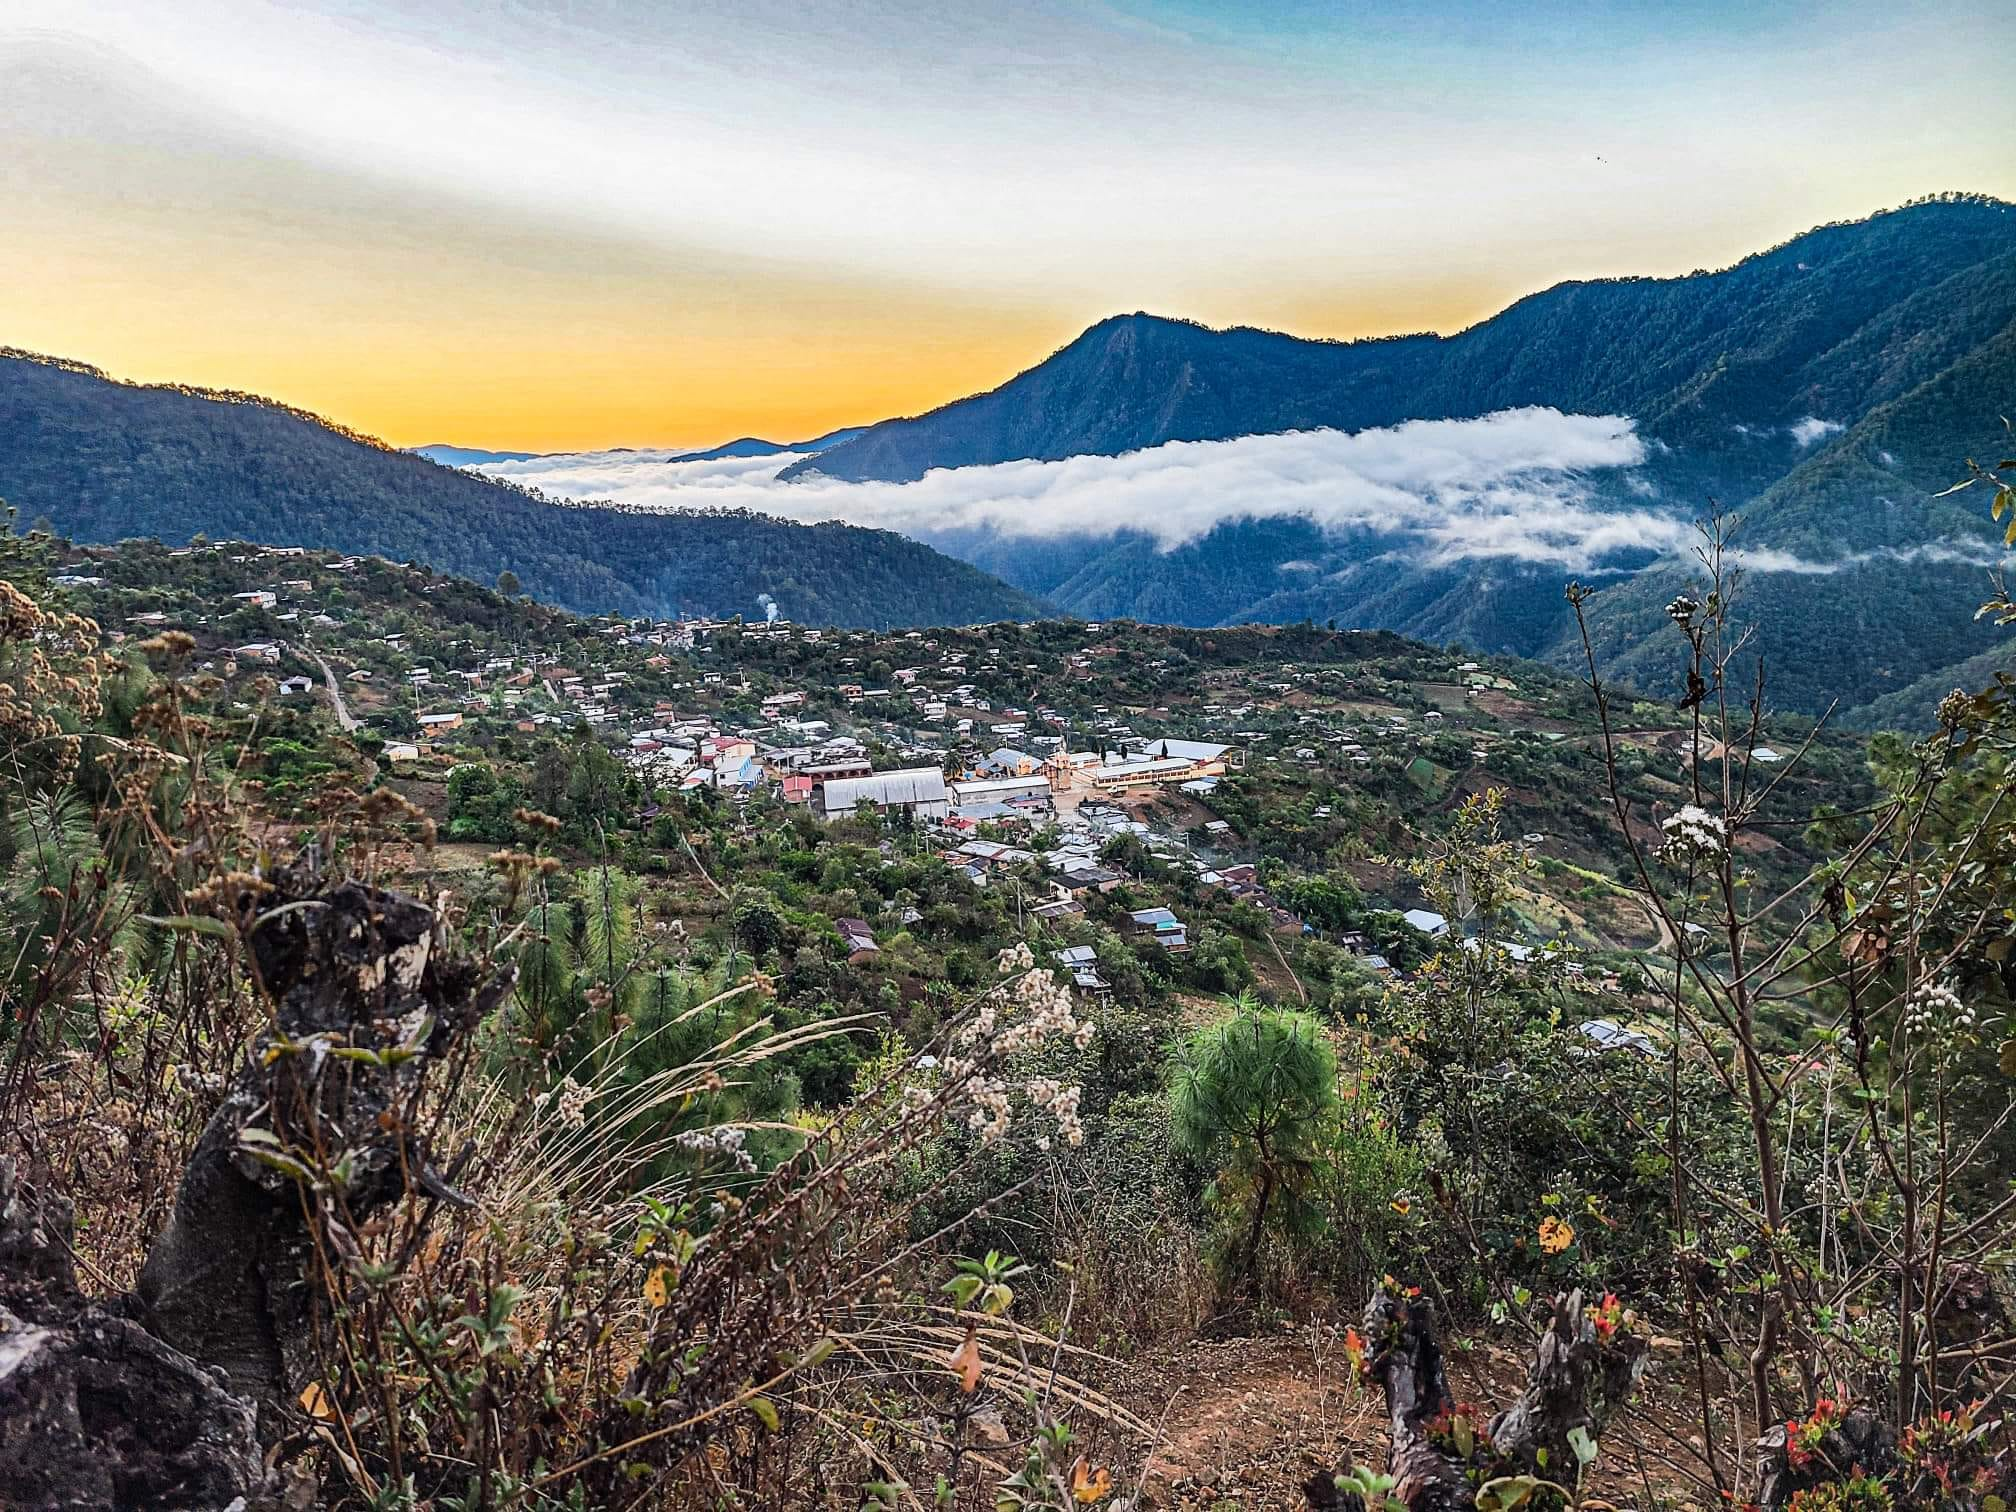
\includegraphics[width=0.9\textwidth]{Images/SantiagoLaxopa.jpeg}
    \caption{Santiago Laxopa taken by Beto Diaz, a resident of Santiago Laxopa.}
    \label{fig:SantiagoLaxopa}
\end{figure}



%-------------------------
\section{Vowels in Santiago Laxopa Zapotec} \label{sec:SLZ-vowels}
%-------------------------

SLZ exhibits a four-vowel inventory; see Table~\ref{tab:SLZvowels}. This type of vowel inventory is very common among Sierra Norte Zapotecs. Most varieties have the vowels /i/, /e/, /a/, and /o/ \citep{nellisFortisLenisCajonos1980,jaegerInitialConsonantClusters1982,butlerh.DiccionarioZapotecoYatzachi1997,avelinobecerraTopicsYalalagZapotec2004,longDiccionarioZapotecoSan2005,sonnenscheinDescriptiveGrammarSan2005}. 

\begin{table}[!h]
    \centering
    \caption{Vowel qualities in Santiago Laxopa Zapotec.}
    \label{tab:SLZvowels}
    \begin{tabular}{lccc}
        \lsptoprule
        &  front& central  & back \\
        \midrule
        high   	&  i  &     &   u$\thicksim$o \\
        mid    	&  e  &   	& 	\\
        low   	&     &  a 	&	  \\
        \lspbottomrule
    \end{tabular}
\end{table}

In SLZ the vowel /o/ is marginal in SLZ's lexicon, only appearing in a few lexical items such as the diminutive classifier \textit{do'}. This vowel is instead replaced by /u/ in most cases. This difference, however, is not universal among all speakers in the community. For the most part older speakers exhibit the vowel /o/ in their speech, while younger speakers tend to replace it with /u/. Most speakers, when asked, classify the two back rounded vowels as the same phoneme and view them as a dialectal feature between the different pueblos. For example, in neighboring San Bartolomé Zoogocho the /u/ vowel is very marginal and has led \citet{sonnenscheinDescriptiveGrammarSan2005} to describe the language as having only four vowels.It is interesting to note that everywhere that SLZ has the vowels /u/ or /o/, Zoogocho only has /o/. Further evidence for this comes from plotting the vowels along the first two formants. As shown in Figure~\ref{fig:SLZvowels}, the vowels /o/ and /u/ occupy nearly identical vowel spaces.

\begin{figure}[!h]
    \centering
    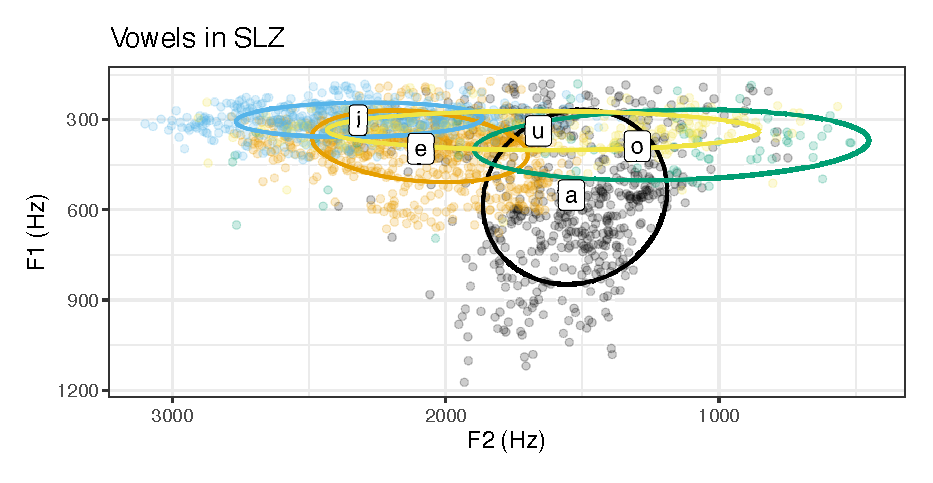
\includegraphics{images/slz_vowels.eps}
    \caption{Vowel space of Santiago Laxopa Zapotec. The ellipses around each vowel mean represents 1 standard. The scale of the axes are in barks with their corresponding Hz values.}
    \label{fig:SLZvowels}
\end{figure}

Additional evidence for the overlap of /o/ and /u/ can be measured with a combination of Pillai scores \citep{pillaiNewTestCriteria1955,hayFactorsInfluencingSpeech2006,nyczBestPracticesMeasuring2014} and Bhattarcharyya's Affinity \citep{bhattacharyyaMeasureDivergenceTwo1943,johnsonQuantifyingOverlapBhattacharyyas2015,warrenQualityQuantityNew2018,strellufChapter3Low2018}. Both of these measures show to what degree of overlap exists between two different items in some space. Their use in linguistics has primarily been used to show the process of a complete and partial mergers between vowels, such as the NEAR-SQUARE vowel merger in New Zealand English \citep{hayFactorsInfluencingSpeech2006}. In the case of SLZ, these measures are used to show that these two vowels are starting to undergo a split. The Pillai scores and Bhattacharyya's Affinity show that the vowels /o/ and /u/ are nearly identical in their vowel space; see Table~\ref{tab:SLZvowels}. In interpreting these results, Pillai scores range from 0 to 1, with 0 indicating overlap and 1 indicating complete no overlap. Bhattacharyya's Affinity ranges from 0 to 1, with 0 indicating no overlap and 1 indicating complete overlap. The results show that the overlap between /o/ and /u/ is not complete, but it is not negligible either.

\begin{table}[!h]
    \centering
    \caption{Pillai scores and Bhattacharyya's Affinity for /o/ and /u/ in Santiago Laxopa Zapotec.}
    \label{tab:SLZvowels}
    \begin{tabular}{lcc}
        \lsptoprule
        &  Pillai score & Bhattacharyya's Affinity \\
        \midrule
        All speakers & 0.157 & 0.892 \\
        Females & 0.138 & 0.890 \\
        Males   & 0.224 & 0.858 \\
        \lspbottomrule
    \end{tabular}
\end{table}
%-------------------------
\section{Voice Quality contrasts in Santiago Laxopa Zapotec} \label{sec:SLZ-voicequality}
%-------------------------
Most Zapotec languages also make use of contrastive voice qualities (see \cite{ariza-garciaPhonationTypesTones2018} for an overview and typology of the voice quality contrasts in the Zapotec language family), with SLZ being no exception. SLZ
has a four-way voice quality contrast: modal, breathy, checked, and rearticulated. These contrasts are exemplified in the minimal quadruple in (\ref{ex:SLZphonation}).

\ea \label{ex:SLZphonation} Four-way near minimal phonation contrast
    \ea \textit{yag}  /çag\supr{L}/ `tree; wood; almúd (unit of measurement approximately 4kg)'
    \ex \textit{yah}  /ça̤\supr{L}/ `metal; rifle; bell'
    \ex \textit{yu'}  /çuˀ\supr{L}/  `cooking pot'
    \ex \textit{ya'a}  /çaˀa\supr{L}/  `market'
    \z
\z
SLZ shares with most Zpaotec varities, two types of creaky voice: checked and rearticulated. Checked vowels are characterized by an abrupt glottal closure which cuts the vowel short. This phonation is sometimes realized as a period of creakiness at the end of the vowel.

Among speakers of SLZ, there is a large amount of inter- and intra-speaker variability in how the rearticulated vowels are produced. Some speakers produce these vowels with a full glottal stop in the middle of the vowel, others produce a vowel with apparent modal voice but with a drop in amplitude (similar to what \cite{gerfenProductionPerceptionLaryngealized2005} found for some Mixtec varities), while others produce creaky voice throughout the entire vowel. Some speakers produce a combination of these unique productions. Overall, these rearticulated vowels are proiduced with some form of manipulation of glottal closure or apmlitude drop in the middle of the vowel.

[INSERT SPECTROGRAMS OF CHECKED AND REARTICULATED VOWELS]

SLZ is unique unique because it is a Northern Core Zapotec that has developed breathy voice, which has not been described in any of the neighboring varieties that make up the Sierra Norte varieties \citep{nellisFortisLenisCajonos1980,jaegerInitialConsonantClusters1982,butlerh.DiccionarioZapotecoYatzachi1997,avelinobecerraTopicsYalalagZapotec2004,sonnenscheinDescriptiveGrammarSan2005,longDiccionarioZapotecoSan2005}.\footnote{Breathy voice in Zapotec languages, however, is common in Central Valley Zapotecs \citep{munroDiCsyonaaryTee1999,espositoSantaAnaValle2004,espositoVariationContrastivePhonation2010,uchiharaToneRegistrogenesisQuiavini2016,ariza-garciaPhonationTypesTones2018}.} Breathy voice is characterized by a raspiness throughout the whole vowel or a portion of the vowel depending on the speaker.

[INSERT SPECTROGRAM OF BREATHY VOWEL]
%-------------------------
\section{Tonal contrasts in Santiago Laxopa Zapotec} \label{sec:SLZ-tones}
%-------------------------
One of the most well known features of all Oto-Manguean languages is the fact that they are tonal languages and exhibit a large range of tonal systems \citep{pikeProblemsZapotecTone1948,renschComparativeOtomangueanPhonology1976,josserandMixtecDialectHistory1983,silvermanLaryngealComplexityOtomanguean1997,beamdeazconaProblemsZapotecTone2007,dicanioItunyosoTrique2010,dicanioCoarticulationToneGlottal2012,elliottChicahuaxtlaTriqui2016,
campbellOtomangueanHistoricalLinguistics2017a,campbellOtomangueanHistoricalLinguistics2017b,
lillehaugenOtomangueanLanguages2019,eischensTonePhonationPhonologyPhonetics2022}. SLZ has a five-way tonal contrast which consists of three level tones (high, mid, low) and two contour tones (rising and falling). 

\citet{brinkerhoffTonalPatternsTheir2022}

%------------------------------------
\section{Interactions between tone and voice quality} \label{sec:SLZ-interaction}
%------------------------------------

% Santiago Laxopa Zapotec (SLZ; \textit{Dilla'xhunh Laxup} [diʒaˀʐun laʂup]) is a Northern Zapotec language spoken by approximately 1000 people in the municipality of Santiago Laxopa, Ixtlán District in the Sierra Norte of Oaxaca, Mexico \citep{adlerAcousticsPhonationTypes2016,adlerDerivationVerbInitiality2018,foleyForbiddenCliticClusters2018,foleyExtendingPersonCaseConstraint2020}.\footnote{This macro variety is also sometimes called Cajonos Zapotec and comprises the dialects of Zoogocho Zapotec, Yatzachi Zapotec, Yalálag Zapotec, Tabaá Zapotec, and Lachirioag Zapotec \citep{smith-starkAlgunasIsoglosasZapotecas2003}.} It is mutually intelligible with San Bartolomé Zoogocho Zapotec \citep{longDiccionarioZapotecoSan2005,sonnenscheinDescriptiveGrammarSan2005}. SLZ has a fairly standard five-vowel inventory; see Table~\ref{tab:SLZvowels}.\footnote{The /o/ vowel is marginal in the lexicon for SLZ and only appears in a few lexical items. In neighboring San Bartolomé Zoogocho the /u/ vowel is very marginal and has led \citet{sonnenscheinDescriptiveGrammarSan2005} to describe the language as having only four vowels. It is interesting to note that everywhere that SLZ has the vowels /u/ or /o/, Zoogocho only has /o/. When plotting the vowel spaces and looking for outliers in the data based on F1 and F2, I noticed that the vowels /o/ and /u/ occupy nearly identical vowel spaces.}


		
% Among Zapotecan languages, it is quite common for languages to make use of contrastive phonation \citep[e.g.,][]{avelinobecerraTopicsYalalagZapotec2004,longDiccionarioZapotecoSan2005,avelinoAcousticElectroglottographicAnalyses2010,lopeznicolasEstudiosFonologiaGramatica2016,chavez-peonInteractionMetricalStructure2010}. In \posscitet{ariza-garciaPhonationTypesTones2018} typological description of phonation in Zapotecan languages, most have two to three phonation types which are described as involving creaky phonation or a glottal closure that is considered a vocalic feature. \citet{ariza-garciaPhonationTypesTones2018} additionally notes that breathy phonation is quite rare among Zapotecan languages, with only three languages in her typological study having this phonation type. Based on this typological data, she claims that breathy phonation is a recent innovation and is restricted to the Valley Zapotec languages only. However, SLZ, as a Northern Zapotec language, presents evidence to the contrary. SLZ has a four-way phonation contrast: modal, breathy, checked, and laryngealized. These contrasts are exemplified in the minimal quadruple in (\ref{ex:YA}).
% \ea \label{ex:YA} Four-way near minimal phonation contrast
%     \ea \textit{yag}  /çag\supr{L}/ `tree; wood; almúd (unit of measurement approximately 4kg)'
%     \ex \textit{yah}  /ça̤\supr{L}/ `metal; rifle; bell'
%     \ex \textit{yu'}  /çuˀ\supr{L}/  `earth'
%     \ex \textit{ya'a}  /çaˀa\supr{L}/  `market'
%     \z 
% \z 

% In representing the checked and laryngealized vowels, I follow the same procedure as other authors (e.g., \citet{avelinoAcousticElectroglottographicAnalyses2010, uchiharaToneRegistrogenesisQuiavini2016}) in representing the ``glottal stop'' element as a superscript glottal stop in the IPA transcription (i.e., [aˀ] or [aˀa]). This is primarily done as a way of standardizing the variable pronunciation of the glottal element in Zapotec, ranging from a full glottal stop (i.e., [aʔ] or [aʔa]) to a creaky portion of the vowel (i.e., [aa̰] or [aa̰a ]).  
% Theoretically, one could argue that checked and laryngealized vowels are not actually phonation types but involve a glottal stop consonant, either as a syllabic onset or coda. It is indeed logical that this could be the case. However, much work has shown that this cannot be true in Zapotec for the laryngealized vowels, which have a glottal closure in their center. \citet{chavez-peonInteractionMetricalStructure2010} summarizes this work and offers six reasons why these ``glottal stops" are a vocalic feature, not a consonant in laryngealized vowels. The first reason has to do with the distribution of the glottal stop. If it is indeed a coda or onset, then we would expect it could also occur word-initially or in consonant clusters. This does not happen in SLZ or other Zapotec languages \citep{jaegerInitialConsonantClusters1982}. Another point that he raises is that when linguists ask native language consultants about how many syllables or beats the word has, they treat laryngealized vowels as if they only had a single beat.\footnote{This is something Maya Wax Cavallaro and I tested with one of our consultants. The only times that they said one of these laryngealized vowels was not a single beat was when they had differing vowel qualities on either side of the glottal closure (e.g., \textit{bi'a} [biˀa] `fly (insect)').} These and other points raised by \citeauthor{chavez-peonInteractionMetricalStructure2010} are presented in (2). 

% \ea  Summary: glottal stop as a vocalic feature in laryngealized vowels (adapted from \cite{chavez-peonInteractionMetricalStructure2010}).
%     \ea /ʔ/ defective distribution (not in onset, not in clusters)
%     \ex Larynealized vowels have the same tonal sequences as single vowels
%     \ex Monosyllabic tendency of the majority of languages (roots = 1σ)
%     \ex *VʔC\sub{fortis}, predicted by bimoraicity of laryngealized vowels
%     \ex Same vowel quality, i.e., one vowel gesture (diphthongs a minority)
%     \ex Perceived as single syllables by native speakers (ʔ ≠ sufficient consonantal barrier, i.e., syllable boundary)
%     \z 
% \z 

% One point that he doesn't mention is that if we assume the glottal stop is a coda consonant, then we would also expect to see the other phonation types being able to co-occur with this coda consonant. Much work still needs to be done from a phonological perspective. Treating /ʔ/ and /h/ as a vocalic feature or as a consonant is worth further study, but in the present work, I assume these sounds are vocalic features and contribute to the phonation contrasts following the traditional interpretation of these sounds. 

% Breathy vowels in SLZ are characterized by a raspiness throughout the whole vowel or a portion of the vowel; see Figure~\ref{fig:BreathyVowel}. For some speakers, it appears as if the breathiness is aligned with the beginning of the vowel and others have it aligned to the end of the vowel. 

% \begin{figure}[!h]
% 	\centering
% 	% [INSERT YAH SPECTROGRAM AND WAVEFORM]
% 	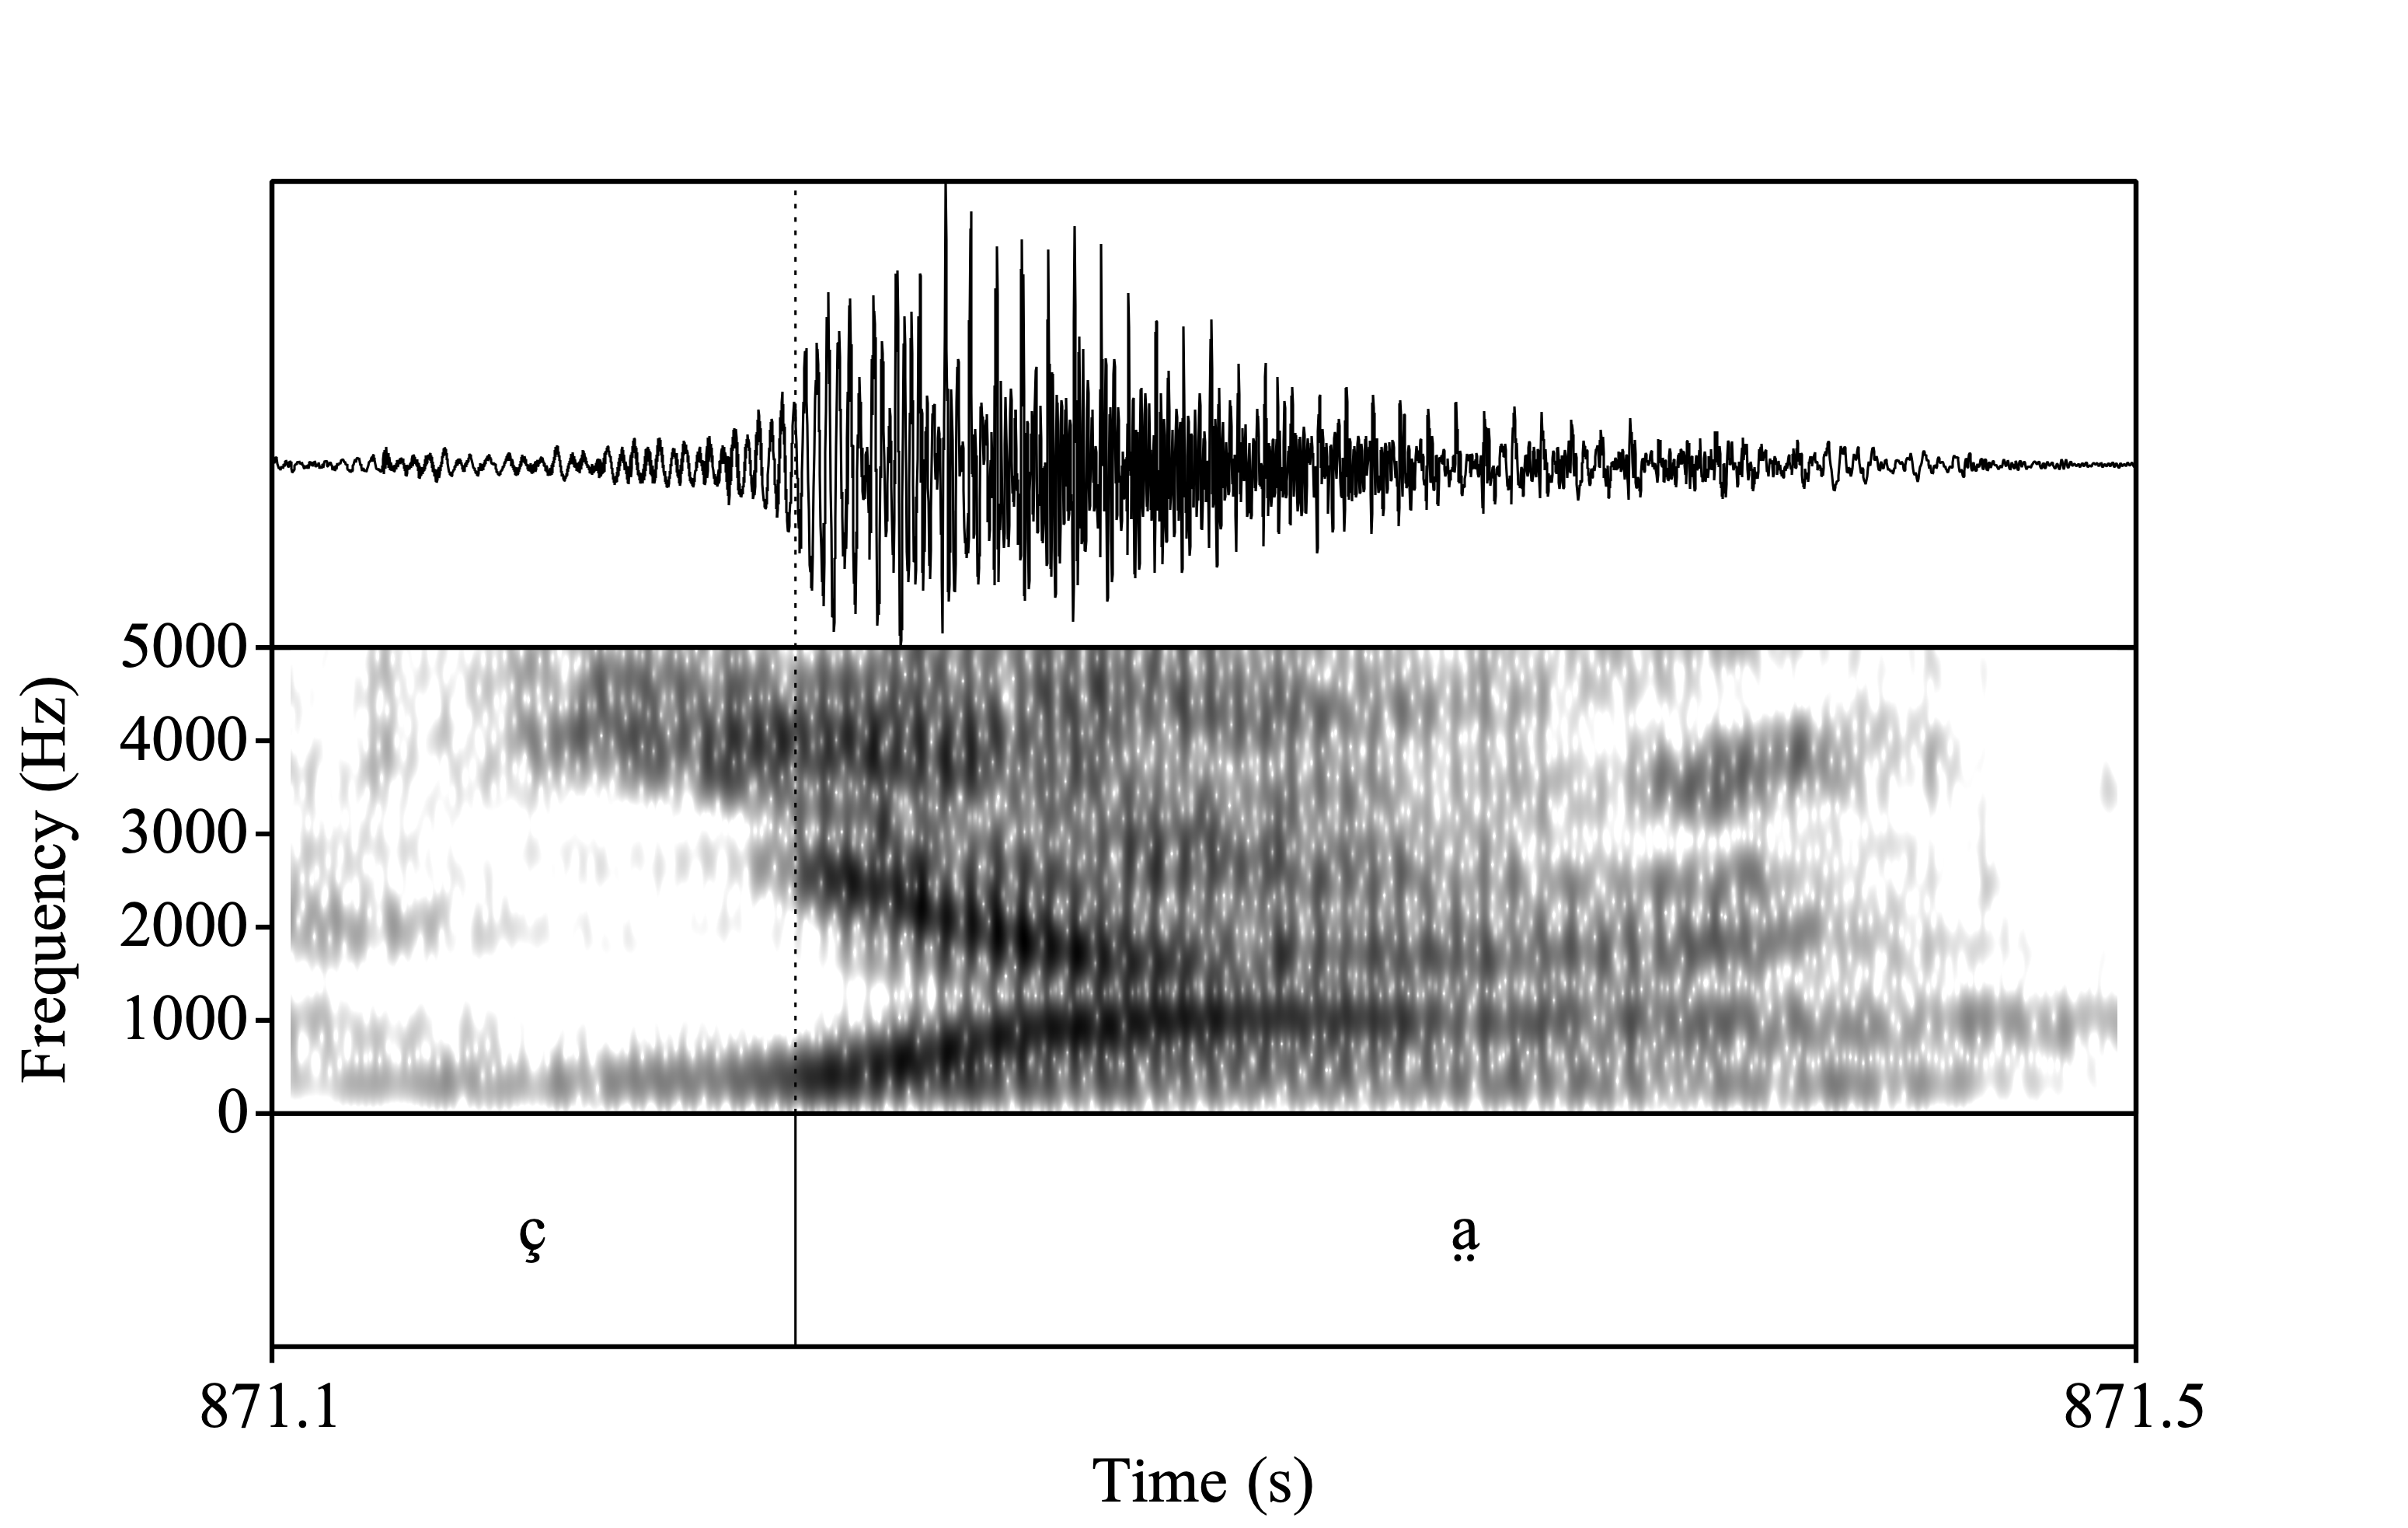
\includegraphics[width=0.9\textwidth]{Images/yah.png}
% 	\caption{Breathy vowel in the word \textit{yah} `metal; rifle'}
% 	\label{fig:BreathyVowel}
% \end{figure}

% On the other hand, checked vowels are characterized by an abrupt glottal closure which cuts the vowel short. This phonation is sometimes realized as a period of creakiness at the end of the vowel; see Figure~\ref{fig:CheckedVowel}.  

% \begin{figure}[!h]
% 	\centering
% 	% [INSERT YA SPECTROGRAM AND WAVEFORM]
% 	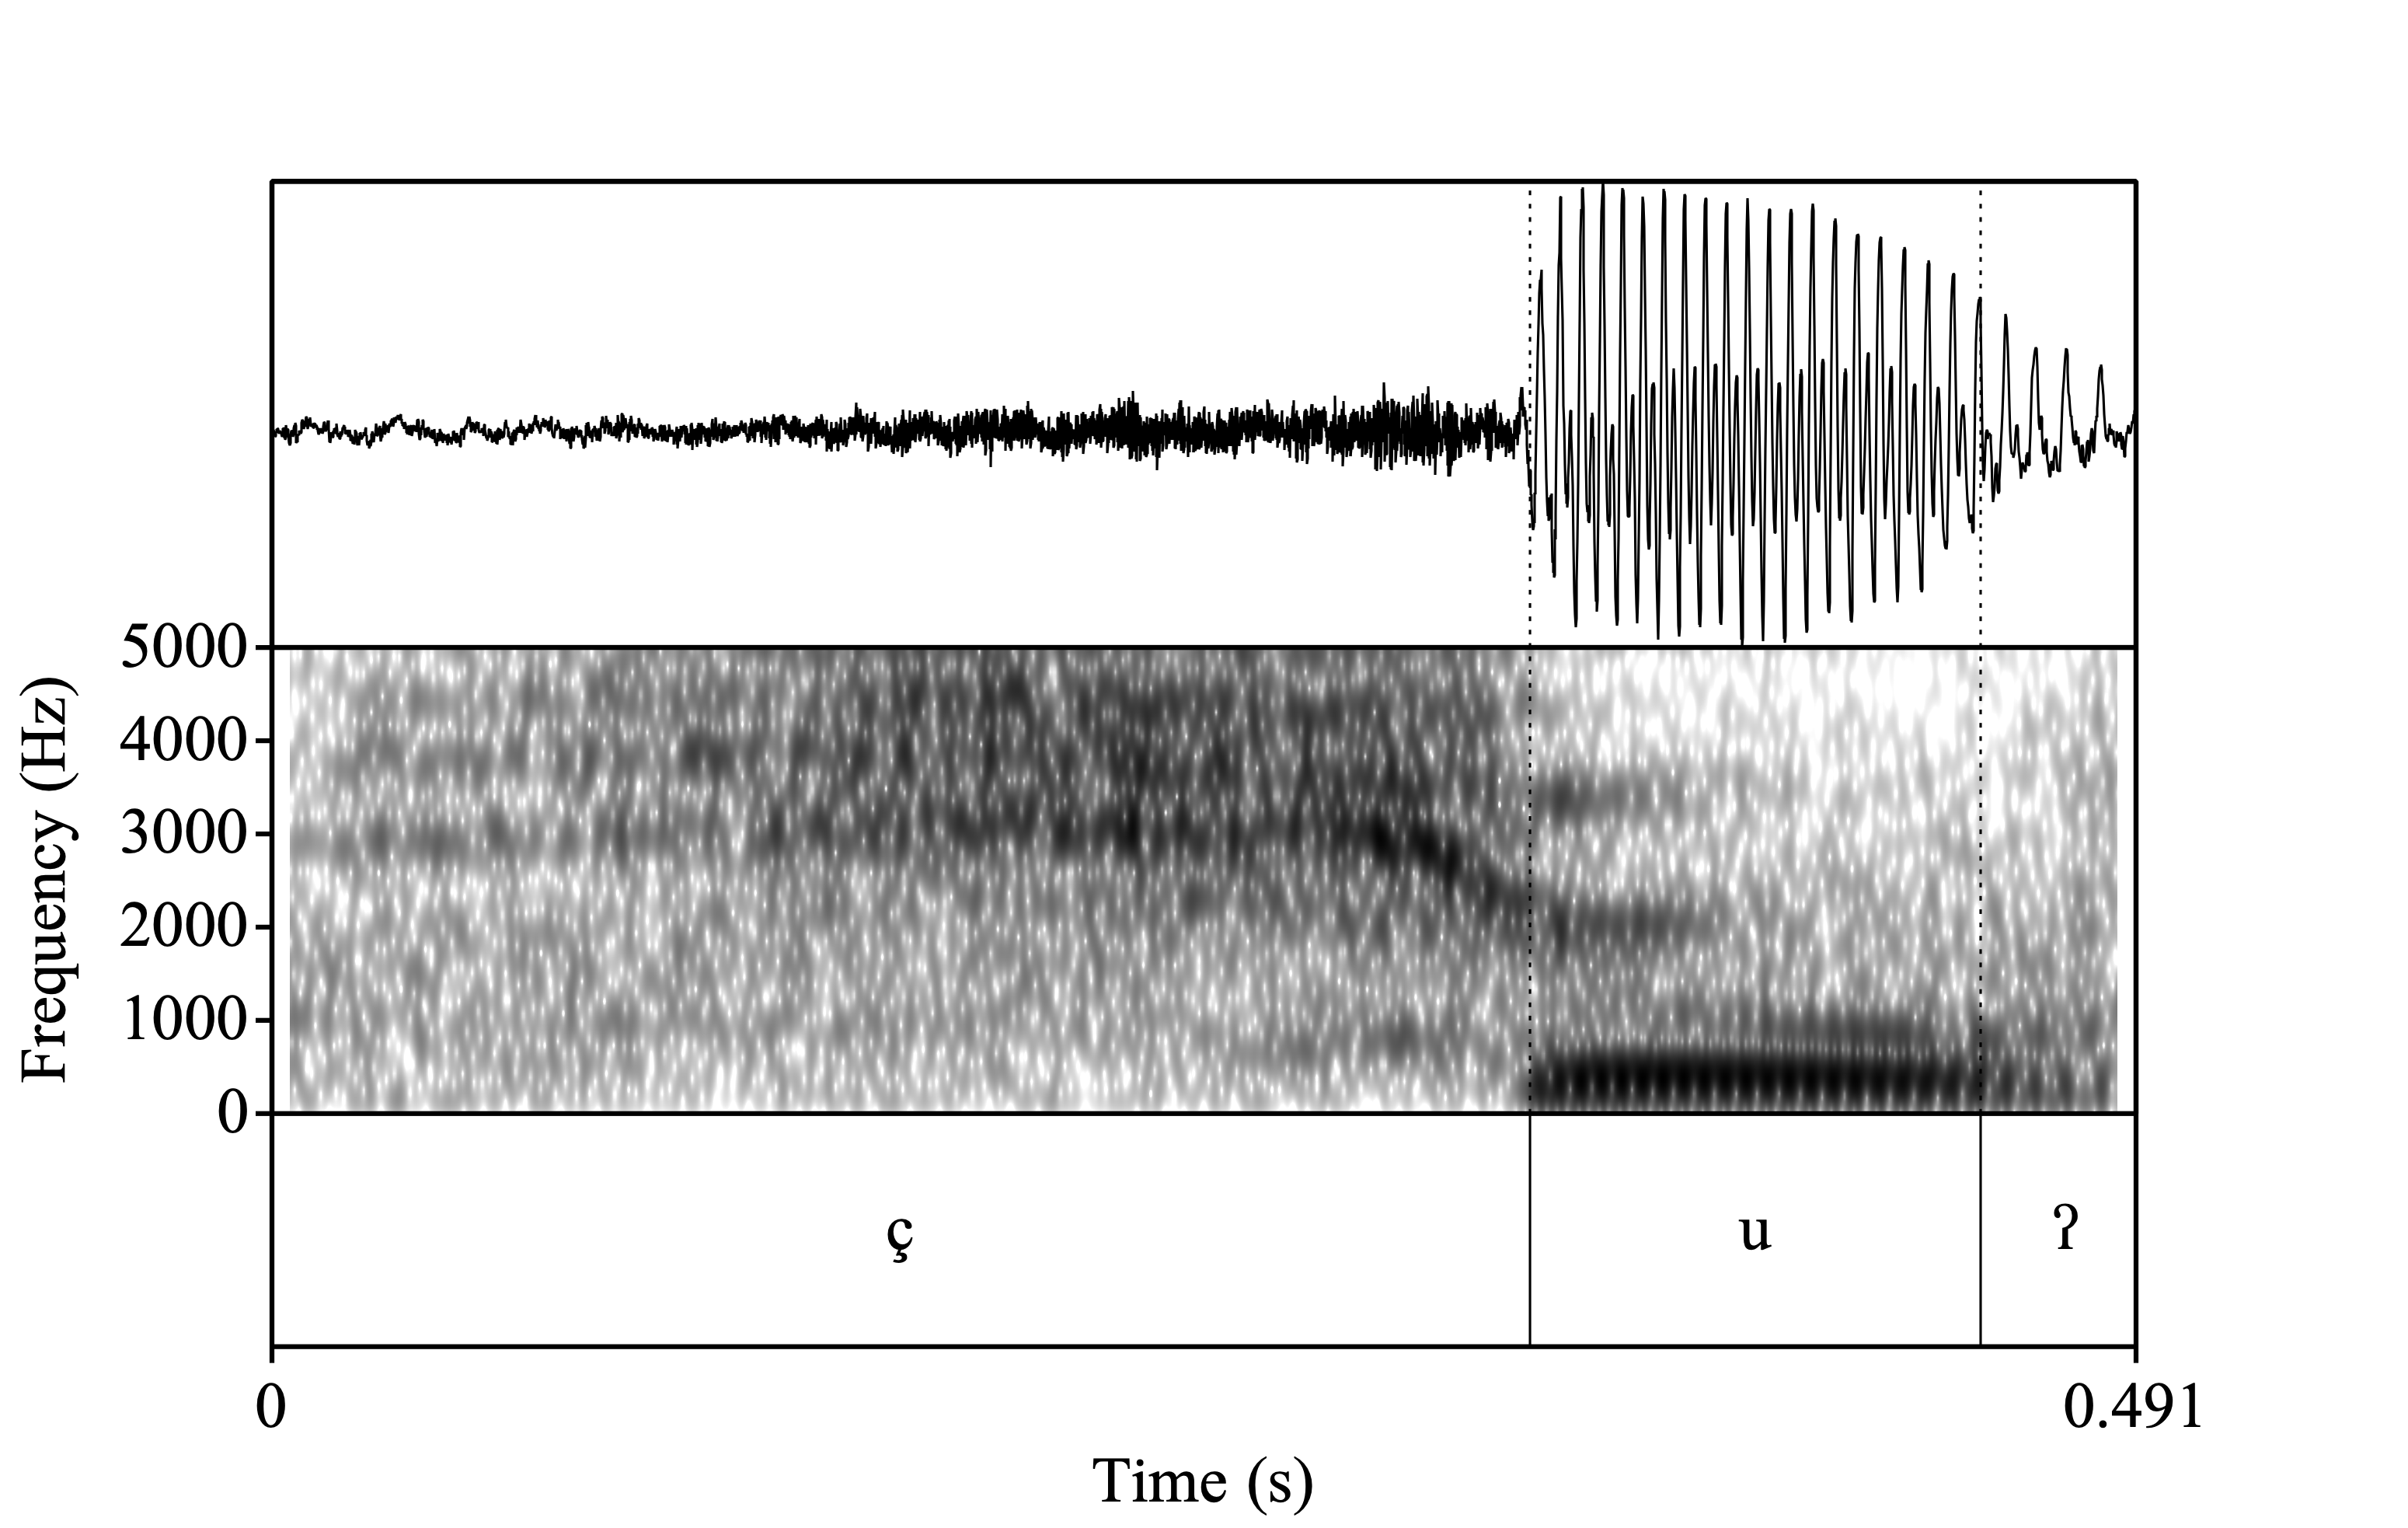
\includegraphics[width=0.9\textwidth]{Images/RD_yu'.png}
% 	\caption{Checked vowel in the word \textit{yu'} `earth'}
% 	\label{fig:CheckedVowel}
% \end{figure}

% Laryngealized vowels are common in Zapotecan languages and have received many names. Previous descriptions have used terms such as broken, rearticulated, interrupted, and creaky to describe this phonation type \citep{longDiccionarioZapotecoSan2005,avelinobecerraTopicsYalalagZapotec2004,avelinoAcousticElectroglottographicAnalyses2010,sonnenscheinDescriptiveGrammarSan2005,adlerAcousticsPhonationTypes2016}. To avoid confusion; I will use the term laryngealized following \citet{avelinoAcousticElectroglottographicAnalyses2010}. In addition to their many different names, these vowels exhibit a wide range of allophones. 

% \citet{avelinoAcousticElectroglottographicAnalyses2010} found in the closely related Yalálag Zapotec that among his consultants, there were at least four different pronunciations as seen in Table~\ref{tab:laryngeal}. 
% \begin{table}[!h]
% 	\centering
% 	\caption{Layngealized Vowels in Yalálag Zapotec}
% 	\label{tab:laryngeal}
% 	 \begin{tabular}{ll}
% 	\lsptoprule
% 	/VˀV/	&  [VʔV]  \\
% 			&  [VV̰V]   \\
% 			&  [VV̰ːV̆]  \\
% 			&  [VV̰V̰]	\\
% 	\lspbottomrule
% 	\end{tabular}
% \end{table}

% In SLZ, this vowel is also highly variable. For most speakers, laryngealized vowels were either creaky throughout their entire production or had a period of creakiness in the middle of the vowel. However, there is a large amount of inter- and intra-speaker variability in how this sound is produced. Some of these other productions included producing modal voice throughout, except for a short period of two or three glottal pulses, which showed a drop in amplitude of five to ten decibels. This drop in amplitude is not too surprising as \citet{gerfenProductionPerceptionLaryngealized2005} showed that this drop in amplitude was sufficient to cue these laryngealized vowels in Coatzospan Mixtec, a member of the Amuzgo-Mixtecan branch of the Oto-Manguean language family. Another frequent production was a complete glottal closure in the middle of the vowel producing a true re-articulation of the vowel. In addition to these productions, combinations of these unique productions were also encountered. Based on my observations, these differences cannot be attributed to sociolinguistic factors (e.g., age, sex, gender, socio-economic status) but seem to be in free variation. 

% To showcase some of these production differences, I show the production of two SLZ speakers who live in Santa Cruz, CA, who participated in piloting this study before I went to Santiago Laxopa for data collection. One of the SLZ speakers in Santa Cruz would re-articulate with a full glottal stop in the middle of the vowel or produce creaky voice. This alternation seemed to be in free variation. Still, there was a greater tendency to creak in low-toned words, such as \textit{xa'ag} [ʂa̰ːg] `topil'\footnote{A \textit{topil} is a type of government office in traditional Oaxacan communities somewhat akin to a sheriff.}, and re-articulate elsewhere; see Figure~\ref{fig:FSRLaryngeal}.

% \begin{figure}[!h]
% 	\centering
% 	\begin{subfigure}{.5\textwidth}
% 		\centering
% 		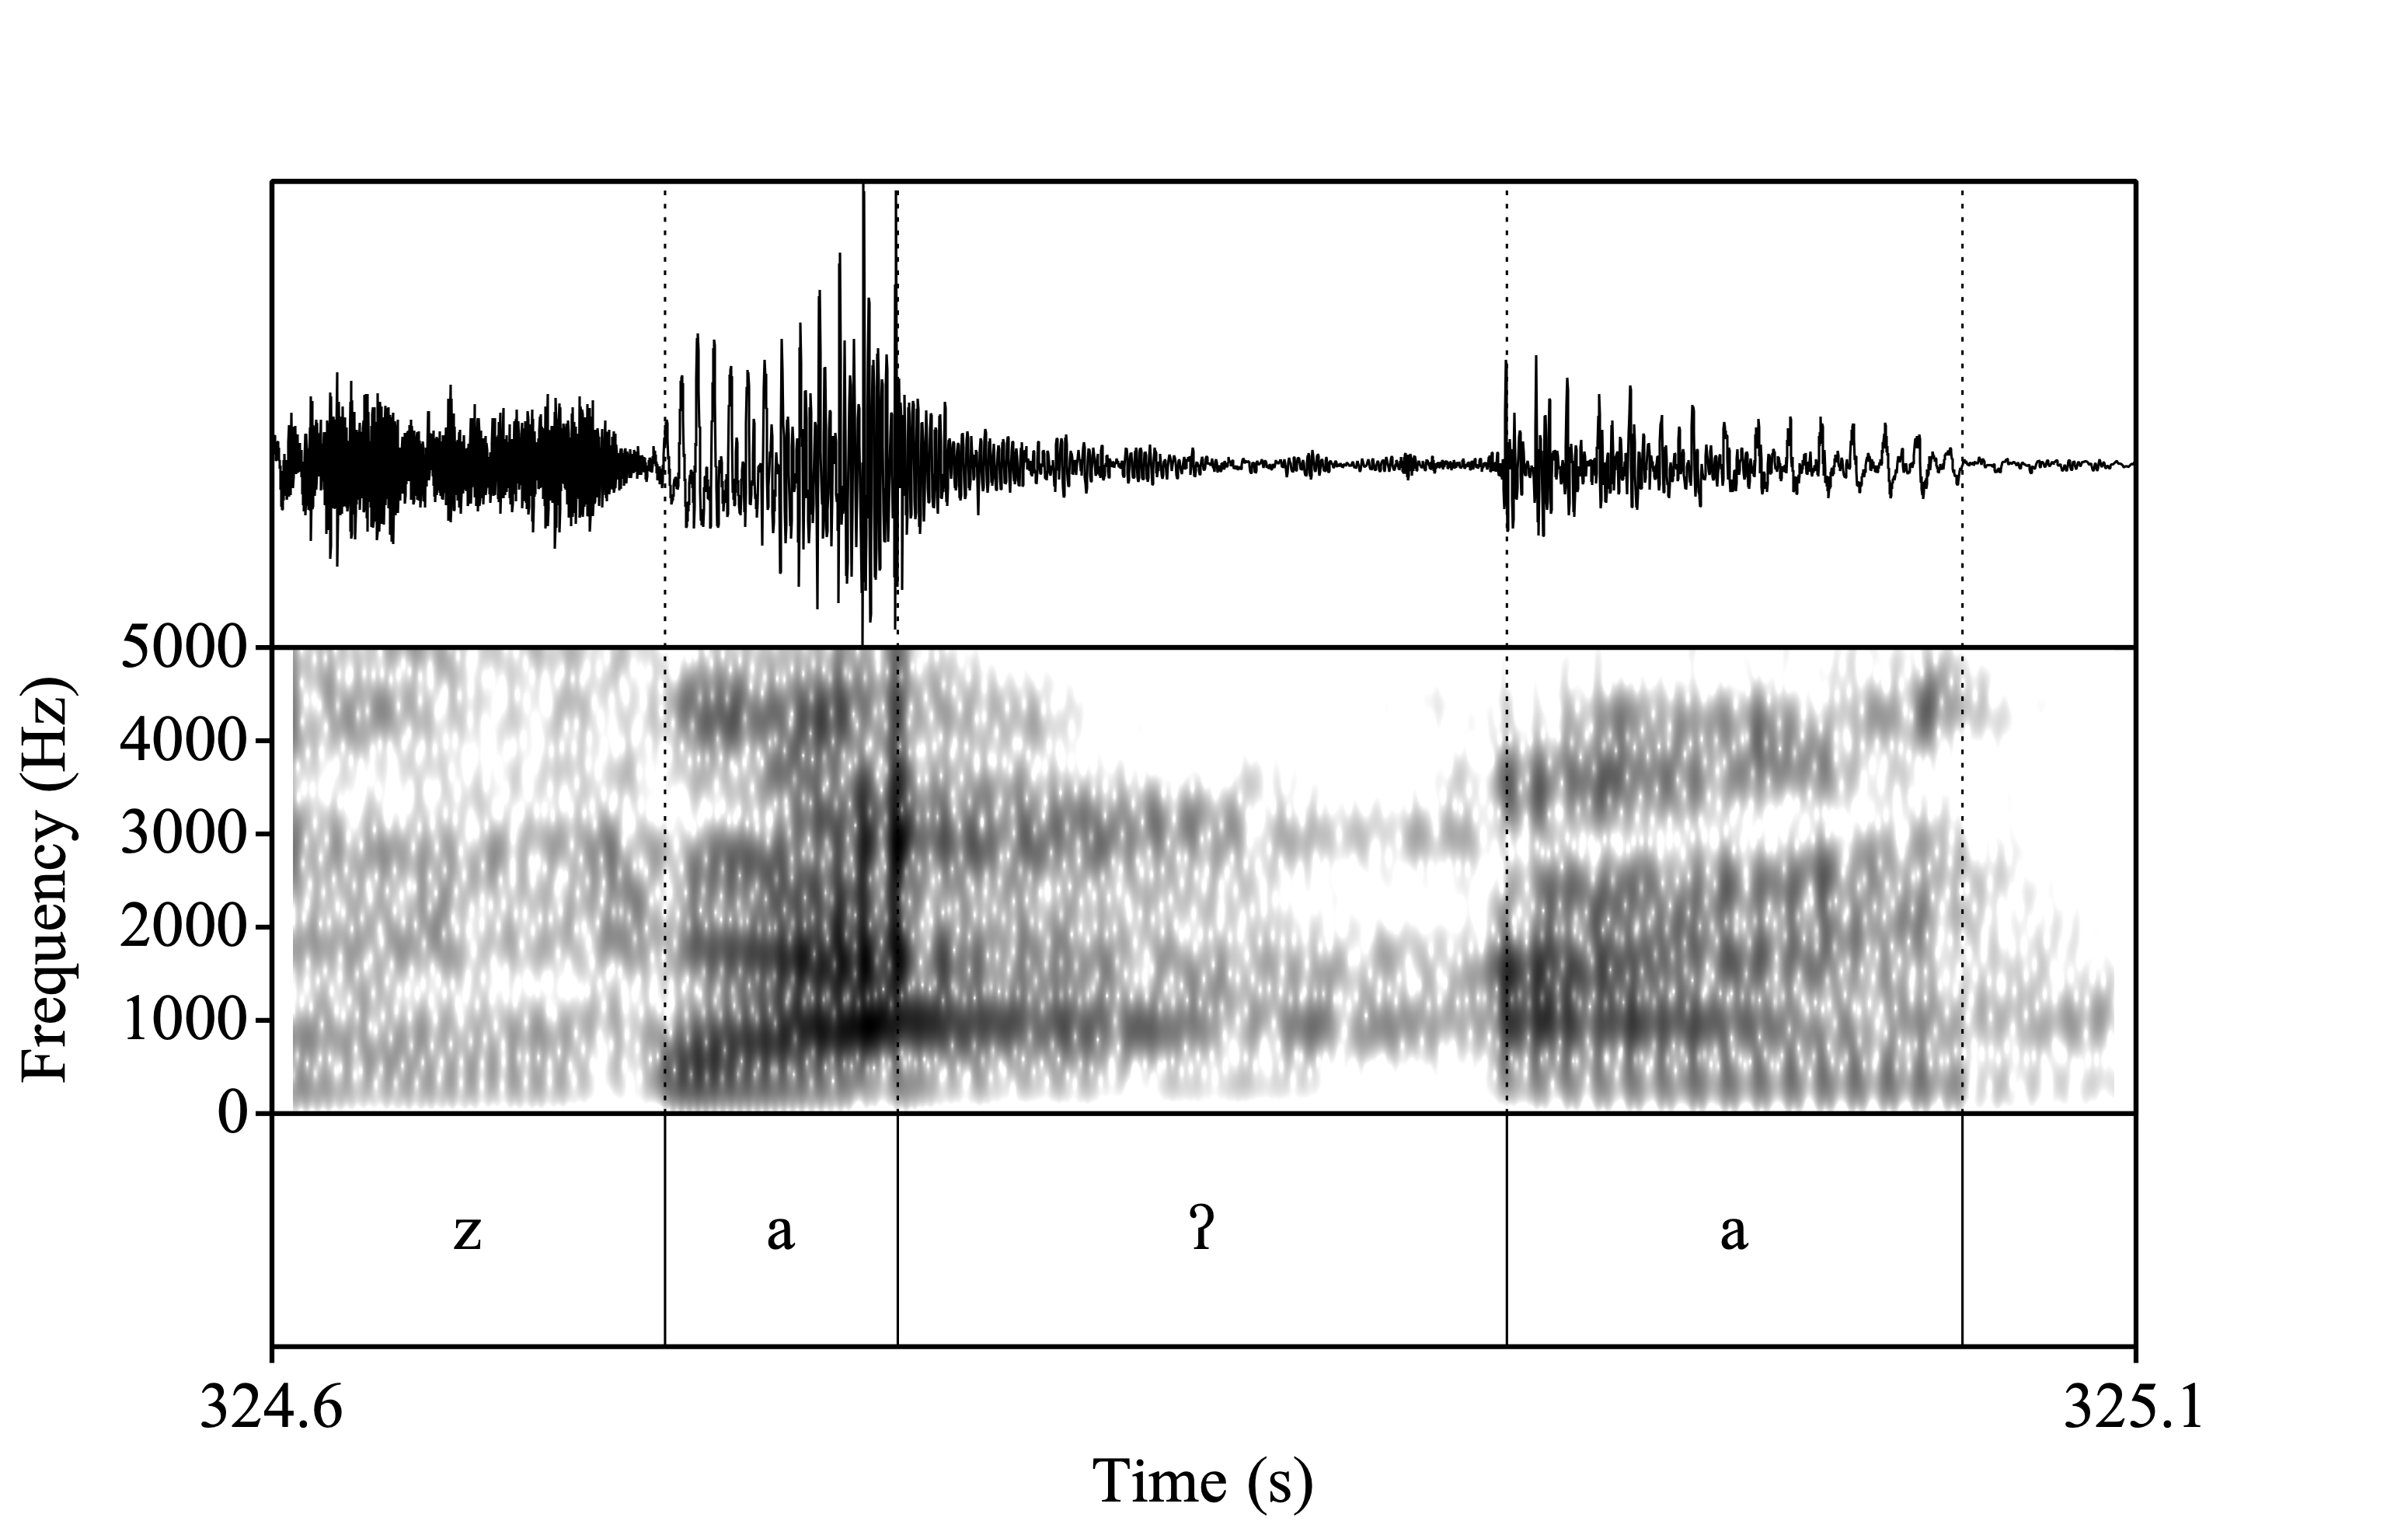
\includegraphics[width=\linewidth]{Images/za'a.png}
% 		\caption{\textit{za'a} `corncob'}
% 		\label{fig:FSRza'a}
% 	\end{subfigure}%
% 	\begin{subfigure}{.5\textwidth}
% 		\centering
% 		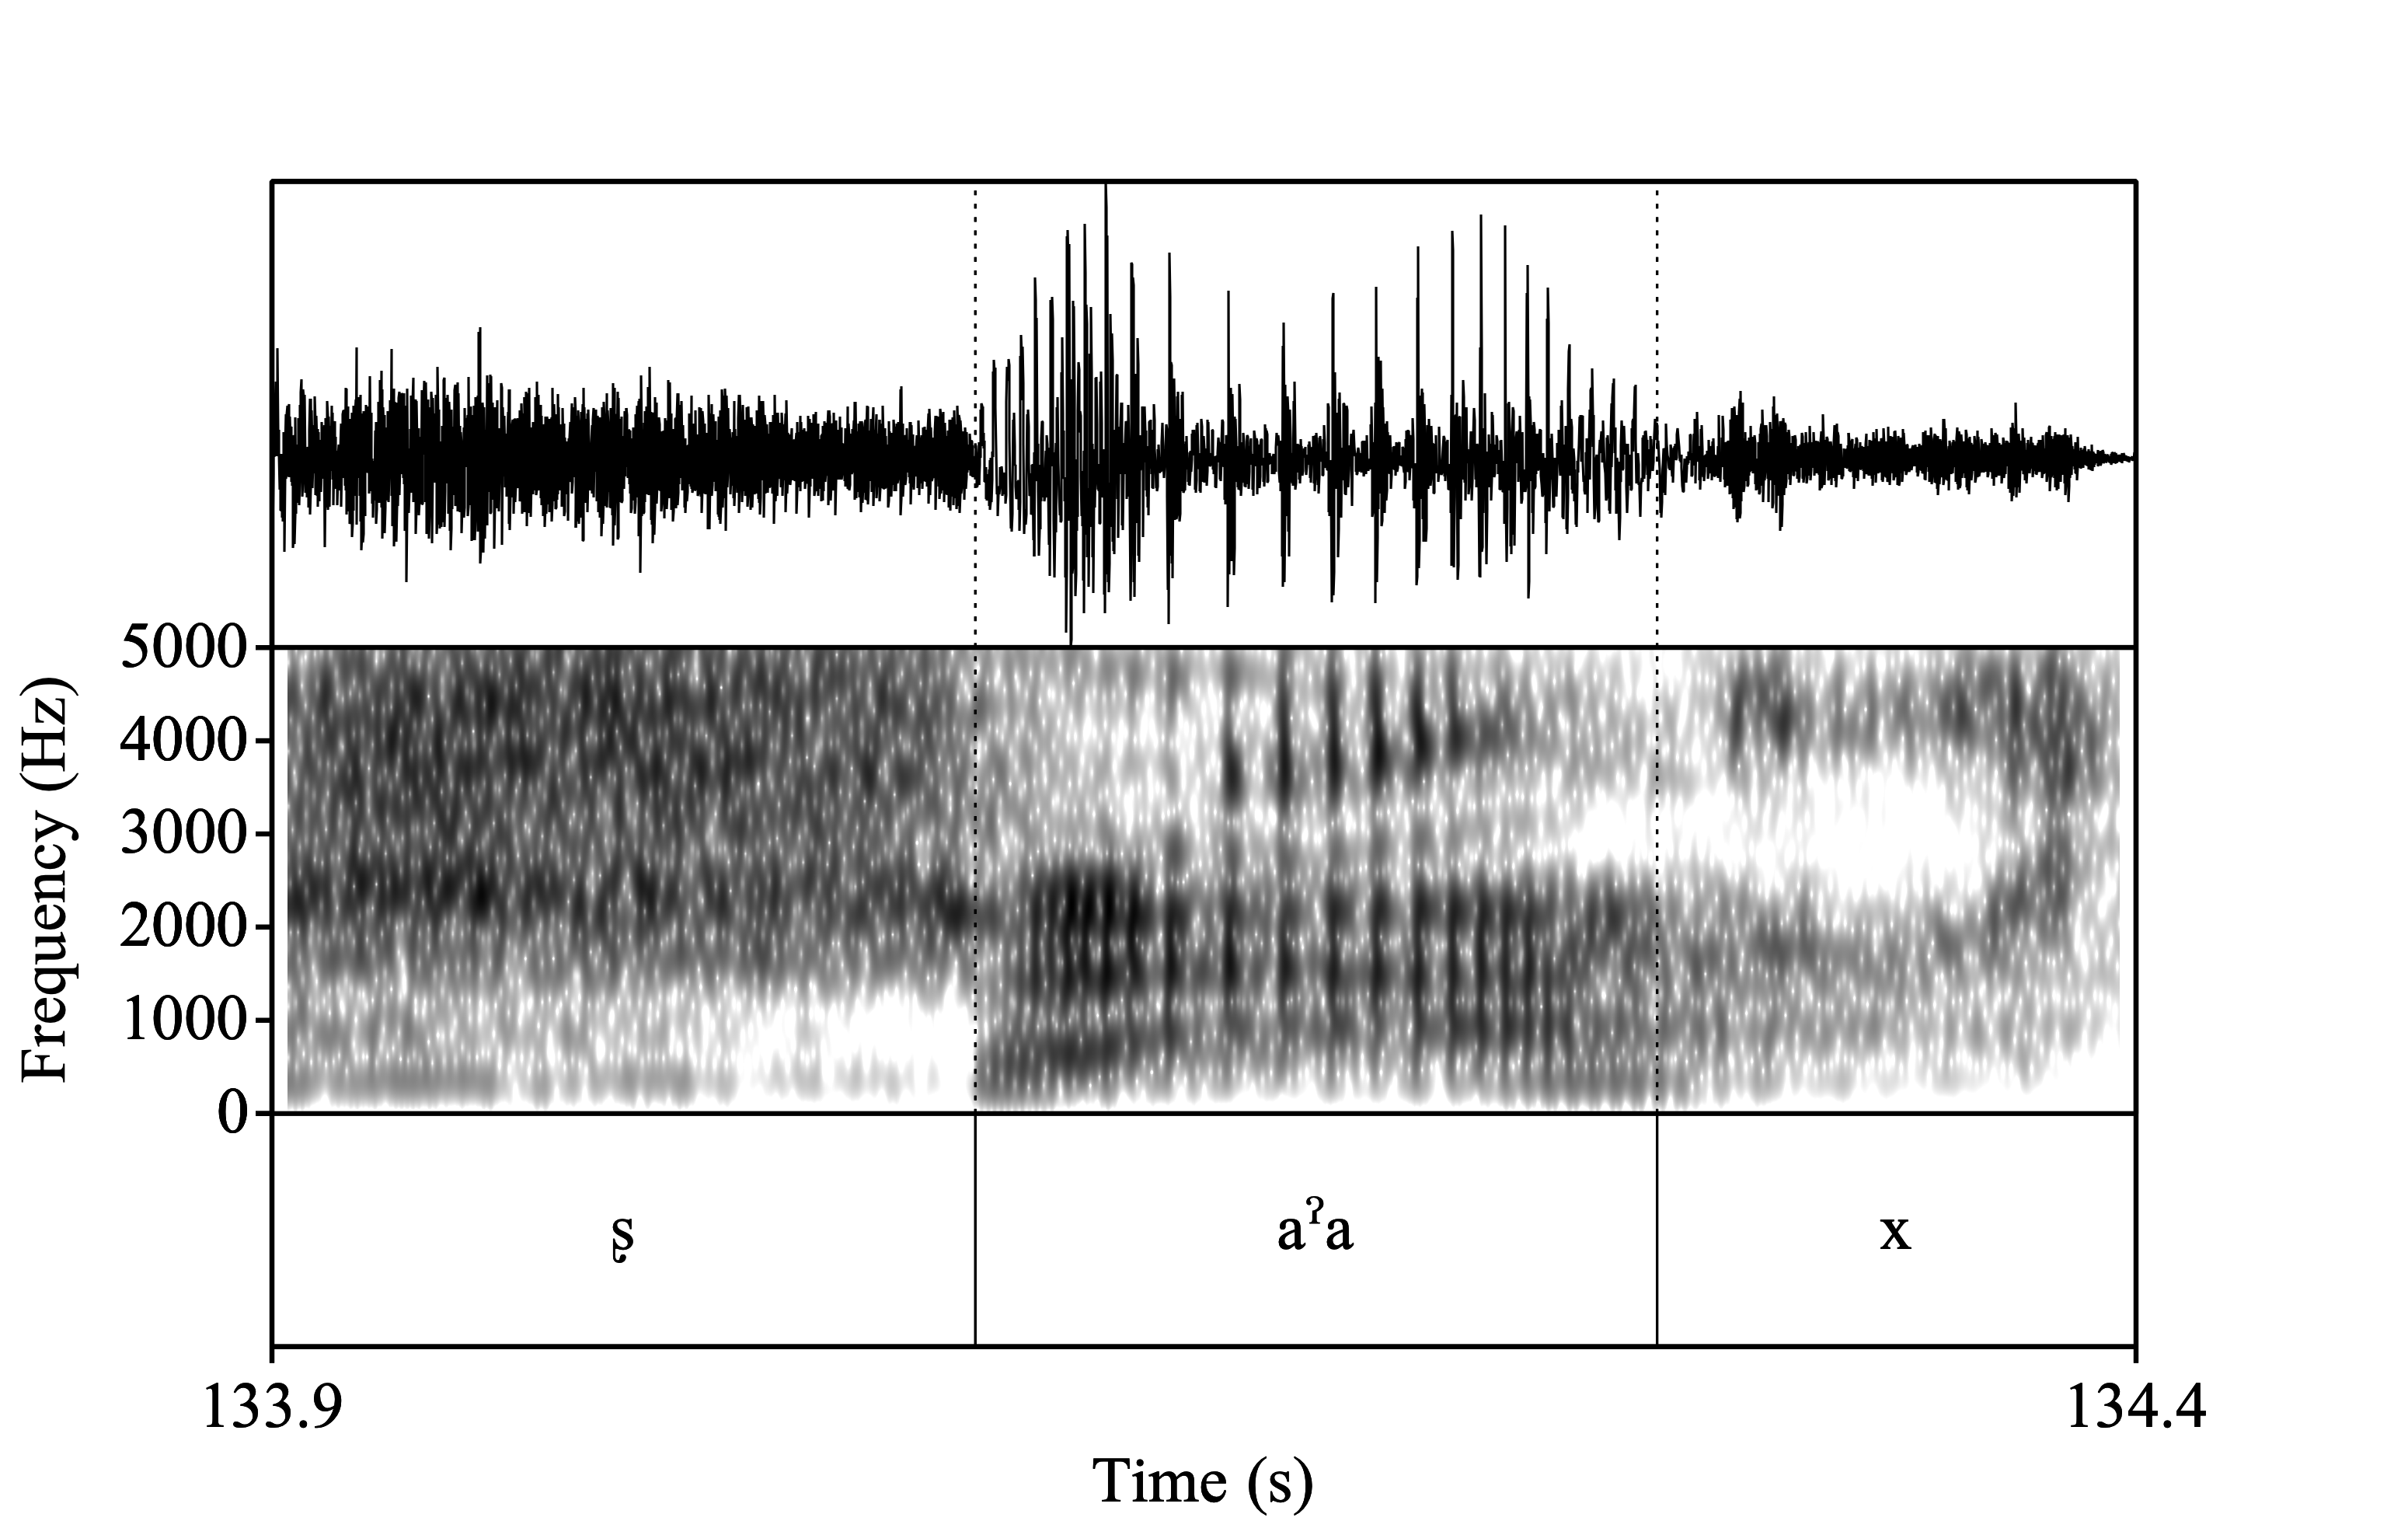
\includegraphics[width=\linewidth]{Images/xa'ag.png}
% 		\caption{\textit{xa'ag} `topil'}
% 		\label{fig:FSRxa'ag}
% 	\end{subfigure}	
% 	\caption{Comparison of FSR's laryngealized vowels in \textit{za'a} `corncob' and \textit{xa'ag} `topil'}
% 	\label{fig:FSRLaryngeal}
% \end{figure}

% The other SLZ speaker only produces creaky voice for these vowels regardless of the tone of the word. During one of the elicitation sessions, my fellow researchers and I conducted a perceptual check that these were, in fact, the same vowels. Both consultants reliably identified the words. They produced laryngealized vowels according to their own idiosyncrasies.
% \begin{figure}[!h]
% 	\centering
% 	\begin{subfigure}{.5\textwidth}
% 		\centering
% 		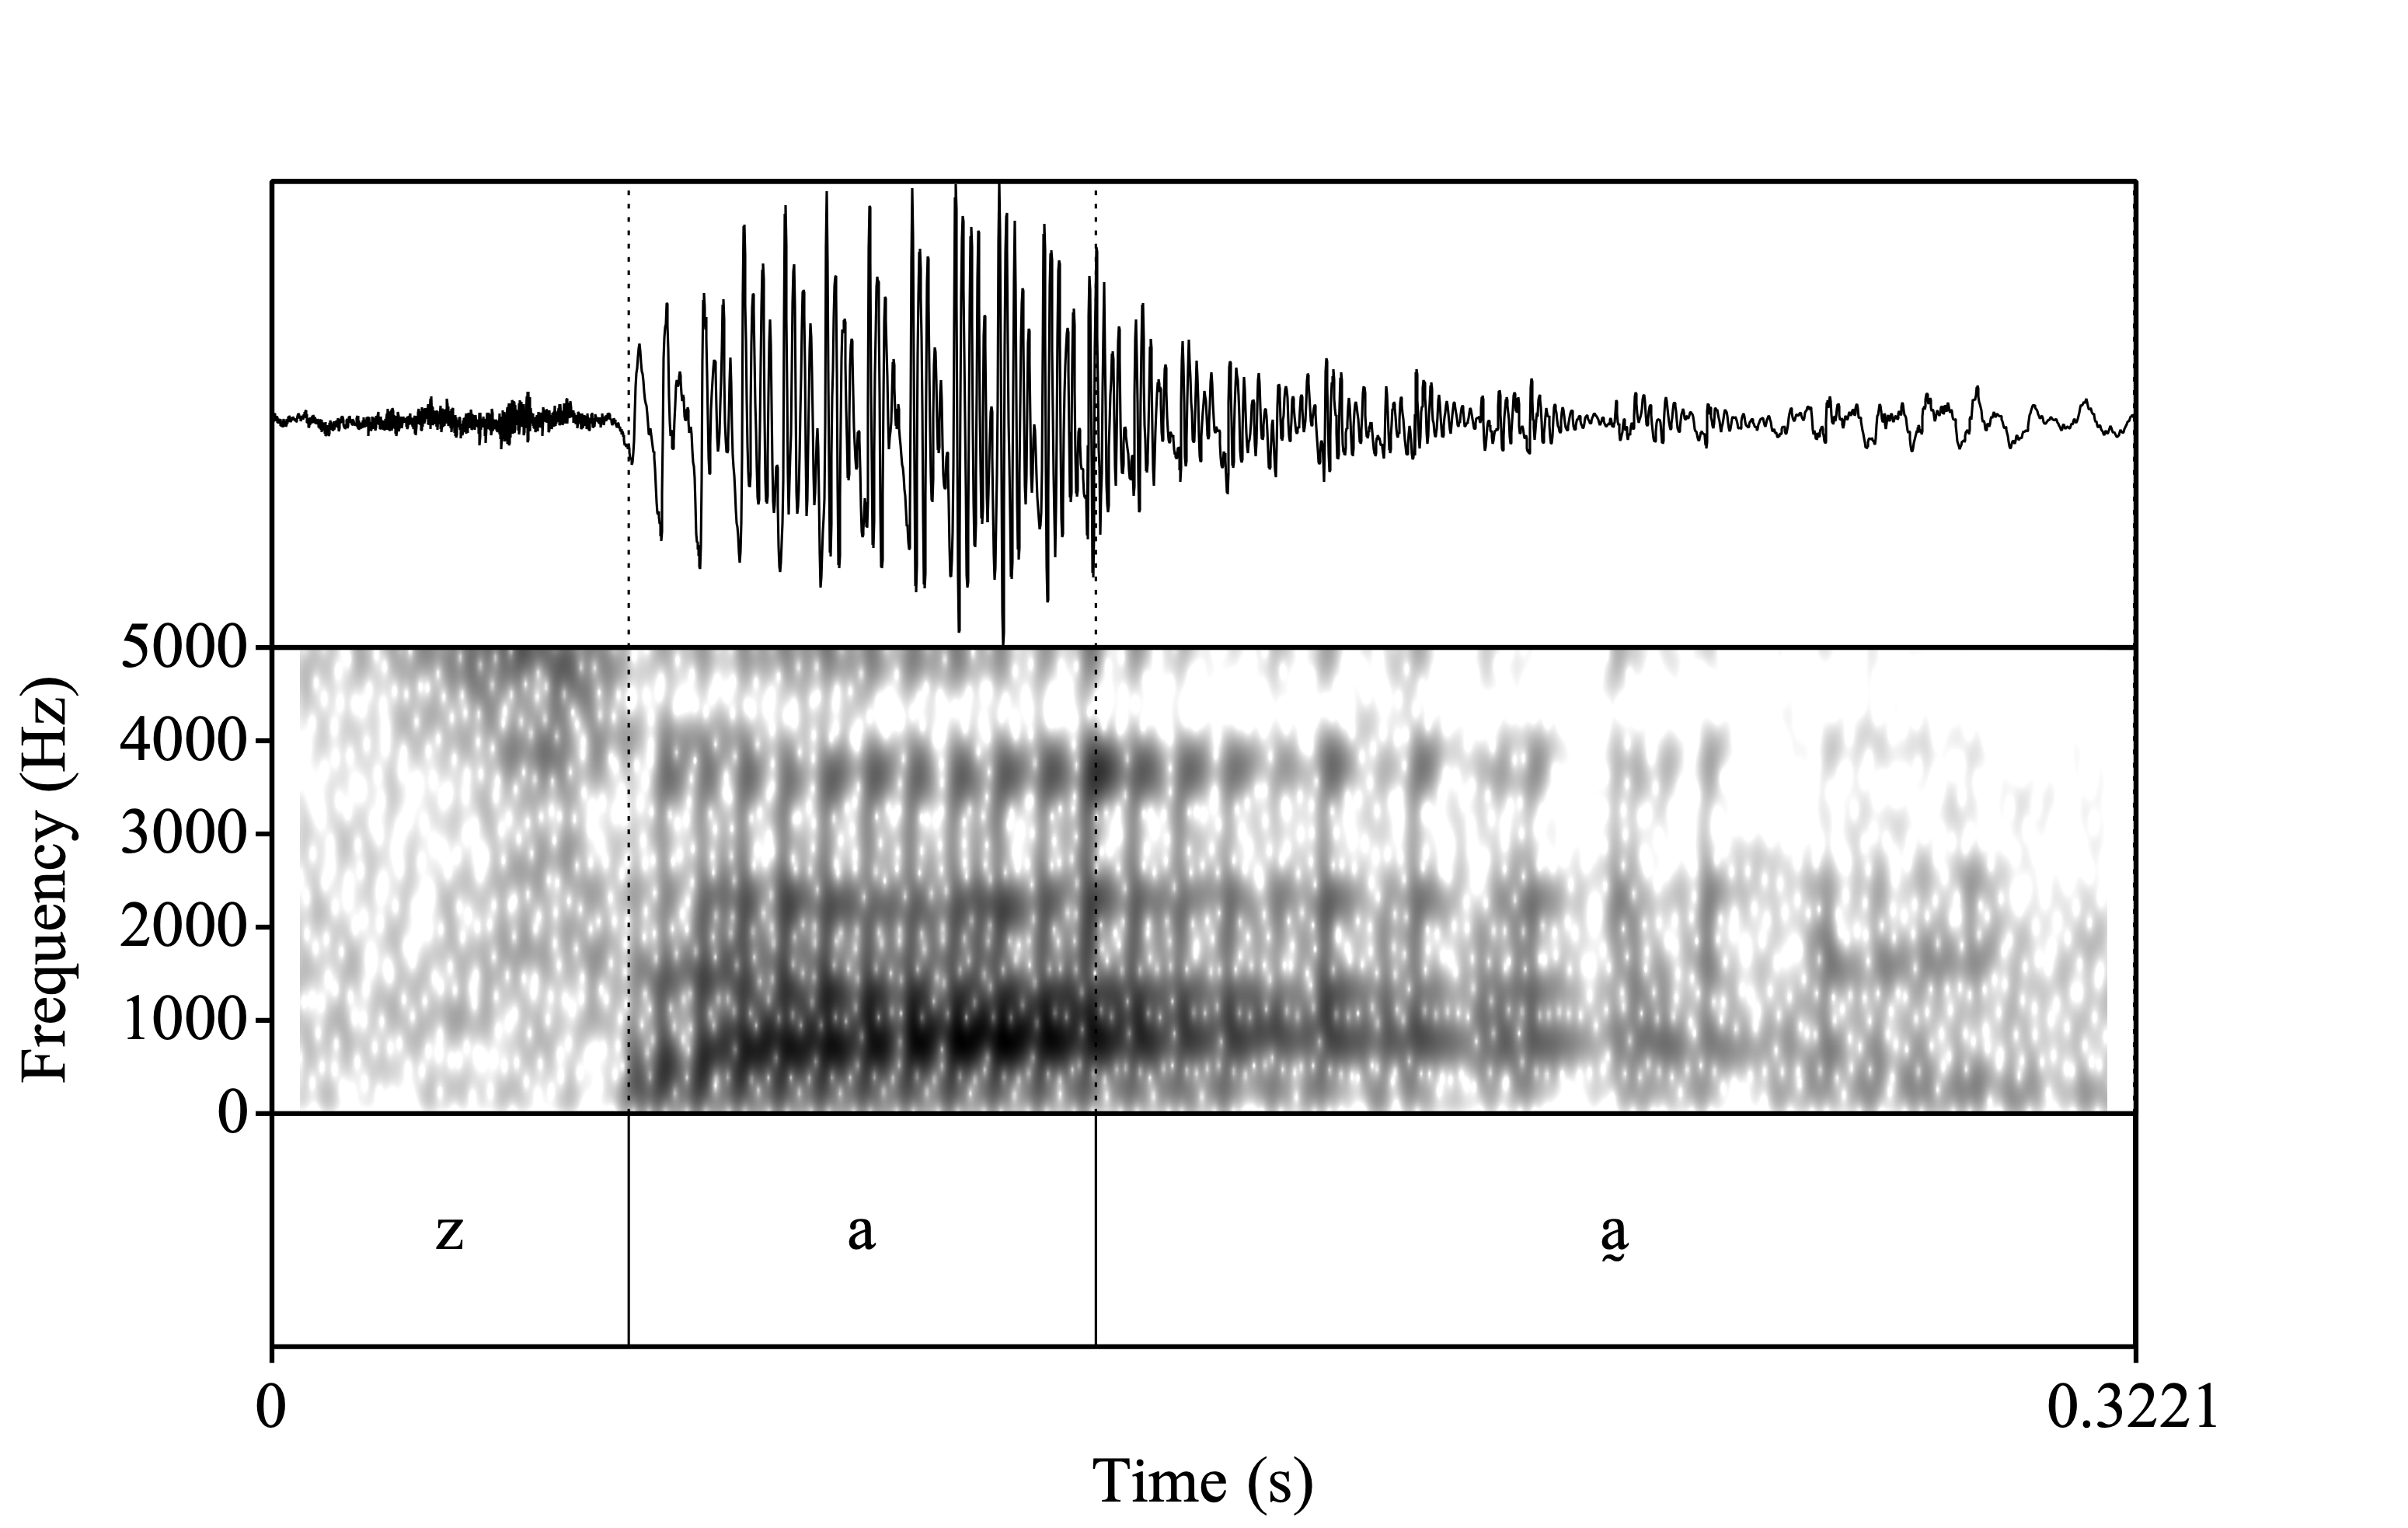
\includegraphics[width=\linewidth]{Images/RD_za'a.png}
% 		\caption{\textit{za'a} `corncob'}
% 		\label{fig:RDza'a}
% 	\end{subfigure}%
% 	\begin{subfigure}{.5\textwidth}
% 		\centering
% 		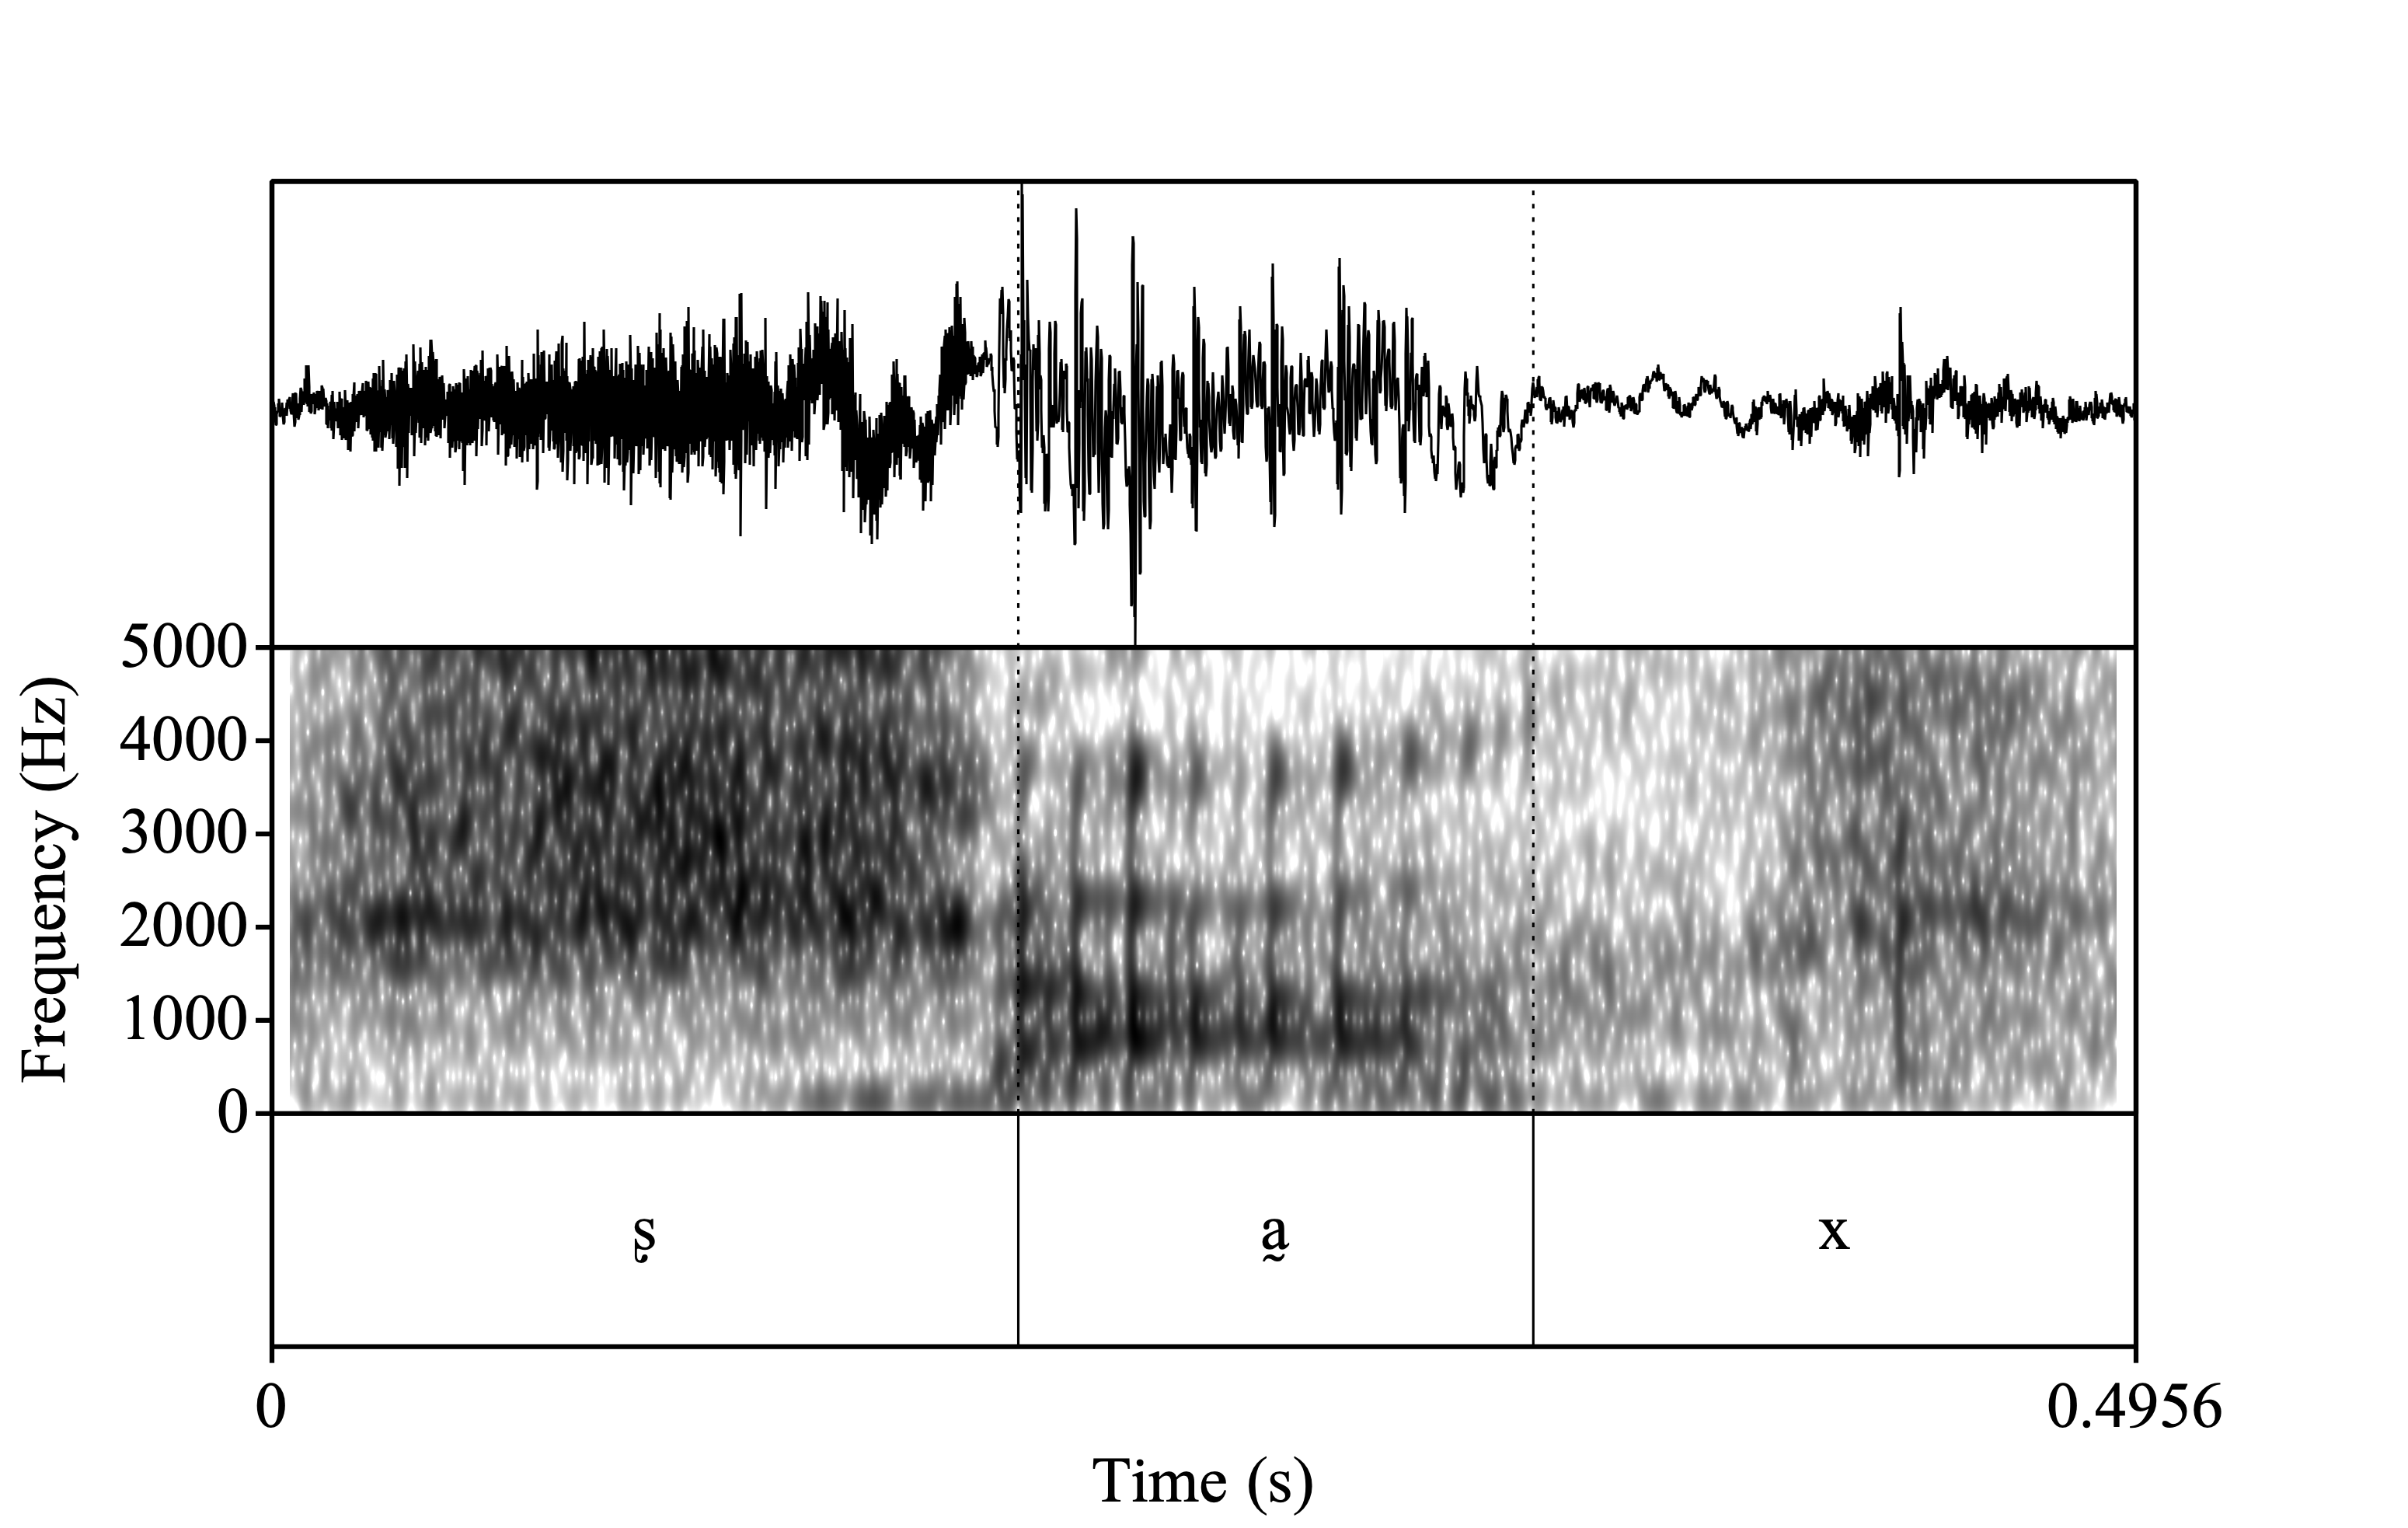
\includegraphics[width=\linewidth]{Images/RD_xa'ag.png}
% 		\caption{\textit{xa'ag} `topil'}
% 		\label{fig:RDxa'ag}
% 	\end{subfigure}
% 	\caption{Comparison of RD's laryngealized vowels in \textit{za'a} `corncob' and \textit{xa'ag} `topil'}
% 	\label{fig:RDLaryngeal}
% \end{figure}

% %------------------------------------
% \subsection{Interaction of Tone and Phonation} \label{sec:Interaction}
% %------------------------------------

% Most previous work on the interaction of tone and phonation has been focused on the languages of East and Southeast Asia (e.g., \cite{masicaDefiningLinguisticArea1976,thurgoodVietnameseTonogenesisRevising2002,yipTone2002,enfieldArealLinguisticsMainland2005,michaudComplexTonesEast2012,brunelleTonePhonationSoutheast2016}). What has been found in these descriptions is that certain tones and phonations are codependent. For example, \citet{smalleyProblemsConsonantsTone1976} and \citet{ratliffMeaningfulToneStudy1992} both describe White Hmong's \textit{-g} tone as being a mid-low tone with breathy phonation, and Mandarin's tone 3 is often associated with creaky phonation \citep{hockettPeipingPhonology1947}. \citet{brunelleTonePerceptionNorthern2009} found that creaky phonation plays an important role in producing certain tones. Additionally, work on S'gaw Karen has found that two tones are only differentiated by some form of non-modal phonation (Boehm p.c.). 

% However, there have been some observations–especially in Mesoamerica–that tone and phonation are independent of each other \citep[e.g.,][]{silvermanLaryngealComplexityOtomanguean1997,garellekAcousticConsequencesPhonation2011}. This means that tone can independently occur with any phonation type. This has also been extensively described in multiple Zapotecan languages \citep[e.g.,][]{,avelinobecerraTopicsYalalagZapotec2004,avelinoAcousticElectroglottographicAnalyses2010, chavez-peonInteractionMetricalStructure2010, campbellZenzontepecChatinoAspect2011,villardPhonologyMorphologyZacatepec2015, lopeznicolasEstudiosFonologiaGramatica2016}

% \citet{chavez-peonInteractionMetricalStructure2010} describes the tone and phonation interactions in San Lucas Quiaviní Zapotec (SLQZ), a central valley variety of Zapotec. The distribution of tone and phonation is found in Table~\ref{tab:SLQZ}. We see that in SLQZ, both low- and falling-tones have the full range of possible combinations. However, we see gaps in the high-tone for breathy and rising tones that can only occur with modal phonation. 

% \begin{table}[!ht]
% 	\centering
% 	\caption{SLQZ tone and phonation interactions \citep{chavez-peonInteractionMetricalStructure2010}.}
% 	\label{tab:SLQZ}
% 	 \begin{tabular}{lcccc}
% 	  \lsptoprule
% 					  &	 \textbf{Modal}  & \textbf{Breathy} & \textbf{Creaky} & \textbf{Interrupted} \\
% 		  High	& ✔︎ & -- & ✔︎ & ✔︎ \\
% 		  Low & ✔︎ & ✔︎ & ✔︎ & ✔︎ \\
% 		  Falling & ✔︎ & ✔︎ & ✔︎ & ✔︎ \\
% 		  Rising & ✔︎ & -- & -- & -- \\
% 	  \lspbottomrule
% 	 \end{tabular}
% \end{table}

Based on elicitation data collected from 2020-2022, SLZ has a more expansive distribution of tone and phonation when compared to SLQZ but seems to be very similar to other Northern Zapotec varieties \citep[e.g.,][]{avelinobecerraTopicsYalalagZapotec2004}. The distribution of SLZ tonal and phonation combinations are given in Table~\ref{tab:ToneVoiceQuality}.
\begin{table}[!h]
	\caption{SLZ tone and voice quality combinations.}
	\label{tab:ToneVoiceQuality}
	\centering

	\begin{tabular}{lcccc}
	\lsptoprule
		& \textbf{Modal} & \textbf{Breathy} & \textbf{Checked} & \textbf{Rearticulated} \\
	\hline
	High		& ✔︎ & -- & ✔︎ & ✔︎ \\
	Mid			& ✔︎ & ✔︎ & ✔︎ & ✔︎ \\
	Low			& ✔︎ & ✔︎ & ✔︎ & ✔︎ \\
	High-Low	& ✔︎ & ✔︎ & ✔︎ & ✔︎ \\
	Mid-High	& ✔︎	& ✔︎ & -- & ✔︎ \\
	\lspbottomrule
	\end{tabular}
\end{table}

% One of the striking things in this is the lack of high tone with breathy phonation. This gap is interesting because of the long-time association of high pitch with breathiness \citep[a good overview–of this association and other phonation types–is found in][]{eslingVoiceQualityLaryngeal2019}. This gap is common across the Zapotecan languages that have breathy voice (Campbell p.c.). Regarding breathy phonation in SLQZ, one of the Valley Zapotec varieties, \citet{uchiharaToneRegistrogenesisQuiavini2016} offers some convincing evidence that the phonation originated in syllables with low tone and then spread to other tones via analogy. Investigating the origin of breathy voice in SLZ would be important in understanding how breathy vowels originated in the Zapotecan family where breathy voice is rare typologically \citep{ariza-garciaPhonationTypesTones2018}. Such a study is beyond the scope of this paper.  
\chapter{The acoustic space of voice quality in Santiago Laxopa Zapotec} \label{ch:acousticlandscape}

%--------------------------------------------------------------------------
\section{Introduction} \label{sec:acousticlandscape:intro}
%--------------------------------------------------------------------------

This chapter studies the acoustic dimension of voice quality in Santiago Laxopa Zapotec (SLZ) using a Multidimensional Scaling (MDS) analysis of acoustic data. MDS is a statistical method that reduces the dimensionality of a dataset and visualizes the relationships between data points. This study uses MDS to visualize the acoustic space of voice quality in SLZ. This analysis provides information on the acoustic correlates of voice quality in SLZ and contributes to our understanding of the phonetic properties of this underdocumented language.

This study is based on the work conducted by \citet{keatingCrosslanguageAcousticSpace2023} on the acoustic space of voice quality in 11 languages. However, this study focuses on a single language, SLZ, and provides a detailed analysis of the acoustic properties of voice quality in this language. The results of this study will contribute to our understanding of the phonetic properties of SLZ and how the acoustic properties of voice quality in this language compare with other languages.

%--------------------------------------------------------------------------
\section{Methods} \label{sec:acousticlandscape:methods}
%--------------------------------------------------------------------------
\subsection{Participants} \label{sec:acousticlandscape:participants}

This study uses data collected from 10 native speakers of SLZ during the summer of 2022. Participants were recruited from the community of Santiago Laxopa, Oaxaca, Mexico. All participants were native speakers of SLZ. The participants were between 18 and 60 years old and consisted of five males and five females.
\subsection{Recordings} \label{sec:acousticlandscape:recordings} 
The participants were asked to perform a word list elicitation task consisting of 72 words. These words were selected to elicit the entire range of types of voice quality in SLZ, including modal voice, the two kinds of creaky (i.e., checked and rearticulated), and breathy voice. The words were selected based on previous research conducted as part of the Zapotec Language Project at the University of California, Santa Cruz \citep{ZapotecLanguageProject}. 
Because participants were not literate in SLZ, the word list was prompted for them by asking them ``How do you say [word in Spanish]?" by myself and another researcher in Zapotec. Participants were asked to respond with the desired word in the carrier phrase \textit{Shnia' [WORD] chonhe lhas} ``I say [WORD] three times.'' which was repeated three times. These utterances were recorded in a quiet environment using a Zoom H4n digital recorder. The recordings were saved as 16-bit WAV files with a sampling rate of 44.1 kHz.

\subsection{Acoustic measuring} \label{sec:acousticlandscape:analysis}
These resulting audio files were then processed in Praat to isolate the vowel portion of each word. The onset of the vowel was set to the second glottal pulse after the onset, and the offset of the vowel was set to the last glottal pulse before the decrease in amplitude at the end of the vowel \citep{garellekAcousticDiscriminabilityComplex2020}. The vowel was then extracted and saved as a separate file for analysis.

These vowels were fed into VoiceSauce \citep{shueVOICESAUCEProgramVoice2009} to generate the acoustic measures for the studies discussed in this dissertation. Because many acoustic measures are based on the fundamental frequency, this measure was calculated using the STRAIGHT algorithm from \citep{kawaharaInstantaneousfrequencybasedPitchExtraction1998}. The STRAIGHT algorithm estimates the fundamental frequency in millisecond (ms) intervals. Once the fundamental frequency is calculated, VoiceSauce then uses an optimization function to locate the harmonics of the spectrum, finding their amplitudes.

VoiceSauce then uses the Snack Sound toolkit \citep{sjolanderSnackSoundToolkit2004} to find the frequencies and bandwidths of the first four formants, also at millisecond intervals. The amplitudes of the harmonics closest to these formant frequencies are located and treated as the amplitudes of the formants. These formant frequencies and bandwidths are used to correct the harmonic amplitudes for the filtering effects of the vocal tract, using \citeauthor{iseliAgeSexVowel2007}'s \citeyear{iseliAgeSexVowel2007} extension of the method employed by \citet{hansonGlottalCharacteristicsFemale1997}. Each vowel was measured across ten equal time intervals, resulting in 22890 data points in total. These measures were then z-scored by speaker to reduce the variation between speakers and provide a way to compare the different measures directly on the same scale.

\subsection{Data processing} \label{sec:acousticlandscape:processing}
Data points with an absolute z-score value greater than three were considered outliers and excluded from the analyses in the dissertation. The Mahalanobis distance was calculated in the F1-F2 panel within each vowel category. Each data point with a Mahalanobis distance greater than six was considered an outlier and excluded from the analysis.  

Energy was excluded if it had a zero value and then log-transformed to normalize its right-skewed distribution. Afterward, the resulting log-transformed data was z-scored, and any data point with a z-score greater than three was excluded. This outlier removal resulted in 1918 data points being removed. 

After removing the outliers, I calculated residual H1* for the remaining data points following \citet{chaiH1H2Acoustic2022}. First, a linear mixed effects model was generated with the z-scored H1* as the response variable and the z-scored energy as the fixed effect. The uncorrelated interaction of the z-scored energy by speaker was treated as random. The energy factor resulting from this linear mixed-effects model was extracted. Finally, the z-scored H1* was the product of the z-scored energy and the energy factor subtracted from it.

Once these steps were completed, the mean of each vowel and speaker of the fifth and sixth intervals was taken. This is similar to what \citet{keatingCrosslanguageAcousticSpace2023} did by taking the middle of the vowel for their analysis. This choice minimizes the effect of the onset and offset of the vowel on the acoustic measures, which are more likely to be affected by the surrounding consonants and should give us the most accurate representation of the vowel quality. Because z-scores were used, this resulted in negative measures, which presents a problem for MDS analyses. To correct for this, I added the absolute value of the minimum z-score to each measure. This results in a dataset that still preserves the relative differences in the scores while providing a dataset that is all positive for the MDS analysis.

\subsection{Statistical analysis} \label{sec:acousticlandscape:statistics}

Using a multidimensional scaling (MDS) analysis is a statistical method of reducing the dimensionality of a dataset to visualize the relationships between the data points \citep{b.kruskalMultidimensionalScaling1978}. This is especially true when many variables could contribute to the data. In the case of voice quality, this is especially true. As shown in \citet{kreimanUnifiedTheoryVoice2014,kreimanValidatingPsychoacousticModel2021,garellekAcousticDiscriminabilityComplex2020}, voice quality is psychoacoustically complex and a single measure is not enough to capture the full range of voice quality. Instead, multiple measures are required that function as cues for the different types of voice quality. For example, a vowel characterized as having a breathy voice has an elevated spectral-slope and a lower harmonics-to-noise ratio than modal voice. A creaky voice has a lowered spectral-slope and a lowered harmonics-to-noise ratio. 

Because MDS analyses that contain many variables can result in rather unmeaningful results, I chose to focus on the speaker x voice quality interaction. This allows us to see how speakers differ in their production of the different voice qualities. This choice to focus on speaker x voice quality means that each speaker's production of each of the four phonation contrasts is represented as a single point in the MDS plot (e.g., one point for speaker 1's modal voice, one for speaker one's checked voice, one for speaker one's rearticulated voice, and one for speaker one's breathy voice). This is similar to what \citet{keatingCrosslanguageAcousticSpace2023} did in their study of the acoustic space of voice quality in 11 languages, except that they compared the language x voice quality interaction. Both of these interactions show us similar information. One shows us within a language, while the other shows us between languages.

The MDS analysis was conducted in R using the  `metaMDS' function in the `vegan' package. The Manhattan distance was used to estimate the physical differences between the speaker x voice quality pairs. Because the distances are non-Euclidean, the MDS analysis was conducted using the non-metric option. 

This algorithm resulted in a solution that involves several different dimensions. The number of dimensions retained directly affects how well the original data is captured. Too many dimensions and the data are overfitted; too few, and the data are underfitted. To determine the number of dimensions to retain, I used a scree plot to plot the stress of each dimension. The elbow of the curve was identified as the correct number of dimensions for analysis. Figure~\ref{fig:stress_plot} shows that most data is captured in a two-dimensional space. The third dimension adds more subtle information about the voice quality.

\begin{figure}[!h]
    \centering
    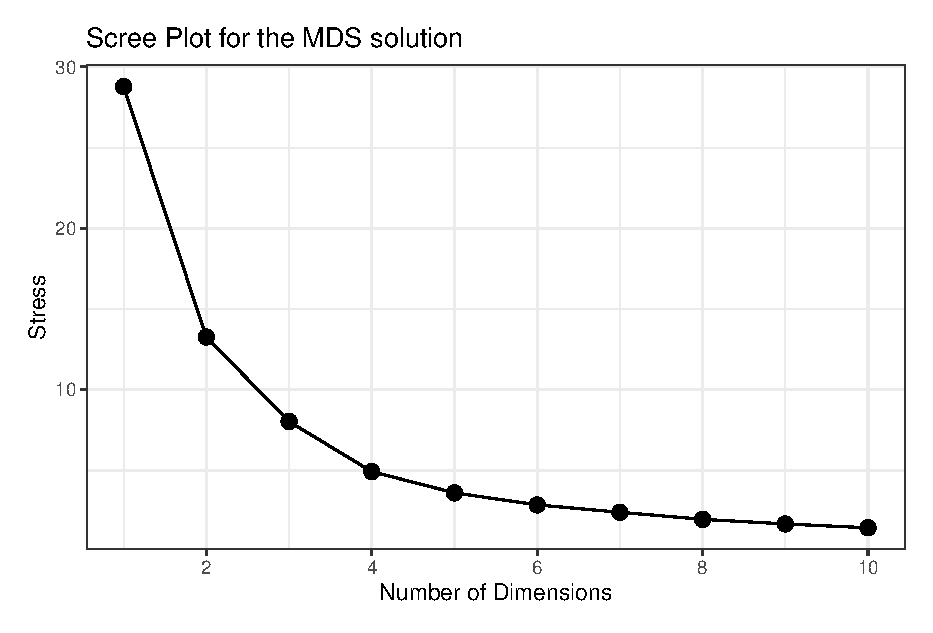
\includegraphics[width = \linewidth]{images/stress_plot.eps}
    \caption{Scree plot for the MDS analysis.}
    \label{fig:stress_plot}
\end{figure}
%--------------------------------------------------------------------------
\section{Results} \label{sec:acousticlandscape:results}
%--------------------------------------------------------------------------
\subsection{Acoustic space of voice quality} \label{sec:acousticlandscape:space}
As mentioned above, the results of the MDS analysis can be represented in a two-dimensional space, as shown in Figure~\ref{fig:nmds12}. In this and all subsequent plots, the breathy voice is represented by black, checked voice with orange, rearticulated voice with green, and modal voice with blue. Overall, we see that the breathy voice is located to the left of the plot, checked and rearticulated voices are tending to the right, and the modal voice is located in the center along the first dimension. The second dimension shows a modal and nonmodal split, with modal voice at the bottom of the plot and nonmodal voice at the top.
\begin{figure}[!h]
    \centering
    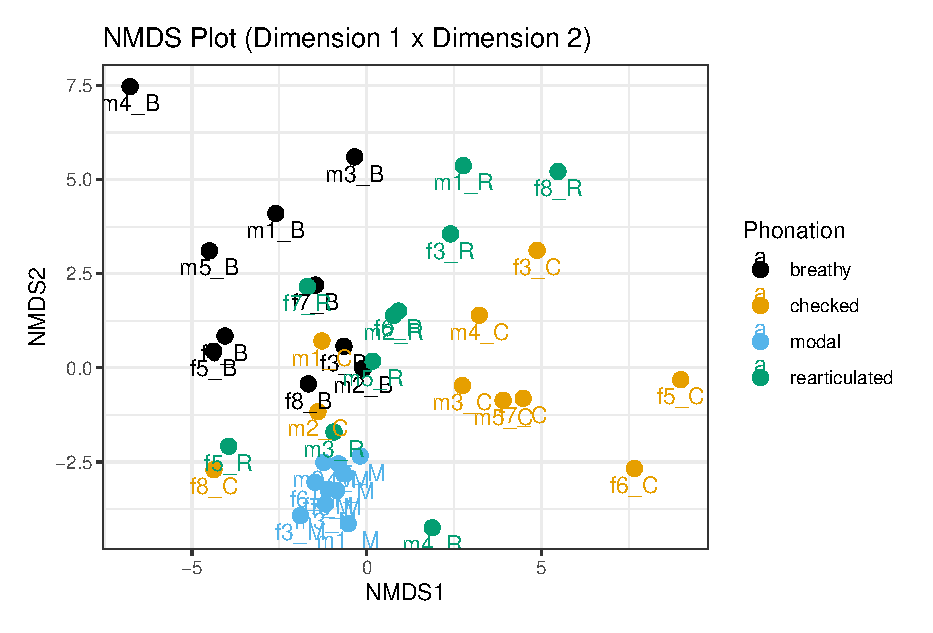
\includegraphics[width = \linewidth]{images/nmds12.eps}
    \caption{Two-dimensional MDS solution showing the first and second dimensions.}
    \label{fig:nmds12}
\end{figure}
    
As mentioned above, the third dimension adds more information about voice quality. Adding the third dimension helps spread the groups along the first dimension, as shown in Figure~\ref{fig:nmds13}. We see that breathy vowels are located at the top of the plot, and the two types of creaky voices (checked and rearticulated) are at the bottom. 

\begin{figure}[!h]
        \centering
        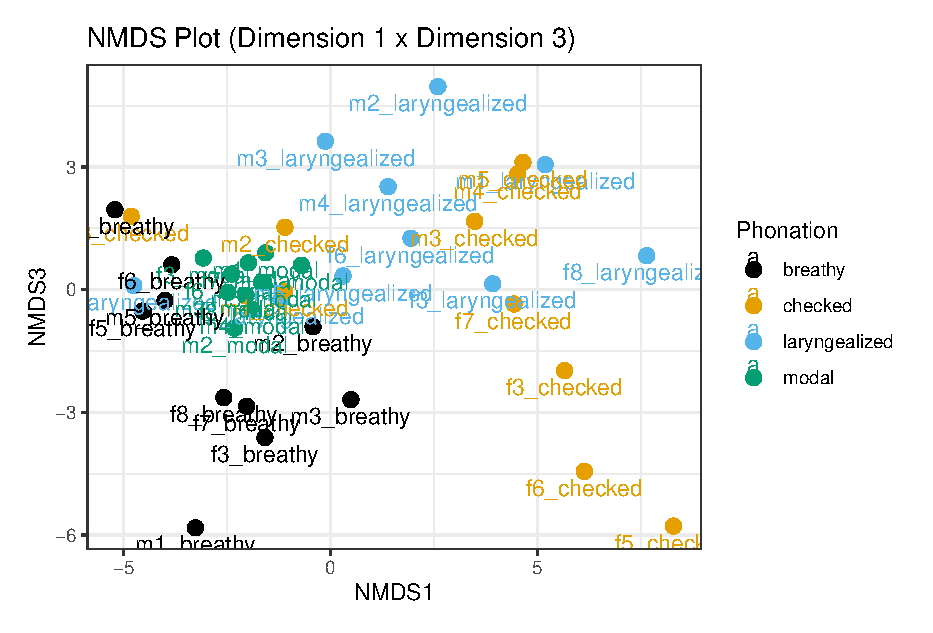
\includegraphics[width = \linewidth]{images/nmds13.eps}
        \caption{Two-dimensional MDS solution showing the first and third dimensions.}
        \label{fig:nmds13}
\end{figure}
    
When adding the third dimension to the second, we see that the breathy voices become separated from the other nonmodal voice qualities, as shown in Figure~\ref{fig:nmds23}. 

\begin{figure}[!h]
    \centering
    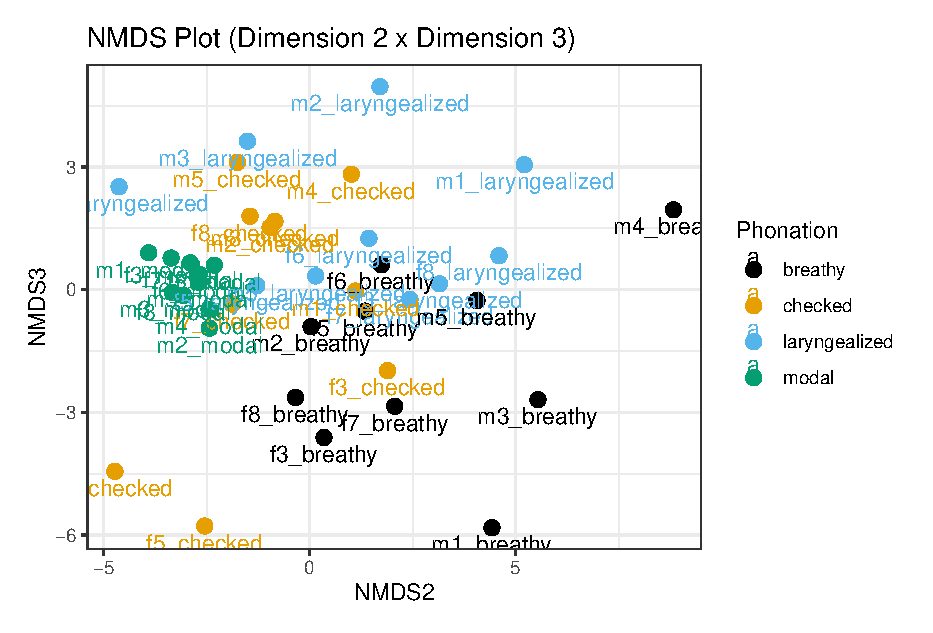
\includegraphics[width = \linewidth]{images/nmds23.eps}
    \caption{Two-dimensional MDS solution showing the second and third dimensions.}
    \label{fig:nmds23}
\end{figure}


\subsection{Acoustic correlates of voice quality} \label{sec:acousticlandscape:correlates}

An additional step to MDS analysis involves testing which acoustic measures contribute the most weight to the different dimensions. Table~\ref{tab:acoustic_correlates} shows the results of this test. In each of the three dimensions of the MDS analysis, the acoustic measures with the highest weight are in bold. In the case of the first and second dimensions (D1 and D2), the acoustic measures that have weights higher than those of other parameters are in boldface (weights > 4.0). In the case of the third dimension (D3), the acoustic measures that have weights higher than those of other parameters are in boldface (weights > 3.0). 

We see that for D1, the acoustic measures that have the highest weight on the first dimension are the amplitudes for the first three formants (i.e., A1*, A2*, A3*) and HNR < 500 Hz (i.e., a harmonics-to-noise ratio for everything from 0 to 500 Hz). For D2, the acoustic measures with the highest weight are H1*-A1*, H1*-A2* (i.e., spectral-slope measures), and the amplitudes of the first two formants. For D3, we see that HNR < 1500 HZ, HNR < 2500 Hz, HNR < 3500 Hz, and Residual H1* and H2* have the highest weights.

\begin{table}[ht]
    \centering
    \caption{Weight of each acoustic measure along each of the three dimensions indicated by the MDS solution (D1, D2, D3). Parameters that have weights higher than other parameters are in bold (weights > 4.0 for D1 and D2, and weights > 3.0 for D3).} 
    \label{tab:acoustic_correlates}
    \begin{tabular}{lrrr}
    \hline
    Acoustic Measure & D1 & D2 & D3 \\ 
    \hline
    h1h2 & 1.03 & 1.01 & 0.39 \\ 
    h2h4 & 1.15 & 3.98 & 2.13 \\ 
    h1a1 & 2.22 & \textbf{5.15} & 1.84 \\ 
    h1a2 & 2.93 & \textbf{4.66} & 1.00 \\ 
    h1a3 & 2.37 & 3.24 & 0.90 \\ 
    h42k & 1.47 & 0.31 & 1.59 \\ 
    h2kh5k & 3.73 & 0.73 & 0.84 \\ 
    h1\_resid & 1.75 & 0.97 & \textbf{4.24} \\ 
    h2 & 1.76 & 0.94 & \textbf{4.09} \\ 
    h4 & 0.79 & 4.28 & 0.10 \\ 
    a1 & \textbf{4.96} & \textbf{5.48} & 0.17 \\ 
    a2 & \textbf{5.30} & \textbf{4.90} & 1.38 \\ 
    a3 & \textbf{4.54} & 2.91 & 1.11 \\ 
    cpp & 4.08 & 0.10 & 1.68 \\ 
    hnr05 & \textbf{5.66} & 1.47 & 1.81 \\ 
    hnr15 & 3.95 & 2.68 & \textbf{3.08} \\ 
    hnr25 & 3.15 & 1.63 & \textbf{3.42} \\ 
    hnr35 & 2.86 & 0.55 & \textbf{3.19} \\ 
    soe & 2.09 & 0.78 & 0.36 \\ 
    shr & 2.39 & 0.50 & 0.47 \\ 
    energy & 2.22 & 3.91 & 0.64 \\ 
    \hline
    \end{tabular}
\end{table}

%--------------------------------------------------------------------------
\section{Discussion} \label{sec:acousticlandscape:discussion}
%--------------------------------------------------------------------------

The results of the MDS analysis show that the acoustic space in which SLZ's voice quality occupies is similar to other languages. Similar to what \citet{keatingCrosslanguageAcousticSpace2023} found in their study, the first dimension appears to roughly be similar to the open quotient of the glottis as proposed by \citet{gordonPhonationTypesCrosslinguistic2001}. In this model, voice quality is seen as the result of the glottis being more open or closed during phonation. The more open the glottis, the more breathy the phonation will be. The more closed the glottis, the more creaky the phonation will be. This model from \citet{gordonPhonationTypesCrosslinguistic2001} is shown in Figure~\ref{fig:phonation_types}.

\begin{figure}[h!]
    \centering
    \begin{tikzpicture}
        % Draw the line with arrows at both ends
        \draw[<->, line width=0.5mm] (0,0) -- (10,0);
        
        % Labels underneath the line
        \node[below] at (0,0) {[h]};
        \node[below] at (2,0) {Breathy};
        \node[below] at (5,0) {Modal};
        \node[below] at (8,0) {Creaky};
        \node[below] at (10,0) {[ʔ]};
        
        % Labels above the line
        \node[above] at (0,0) {Open Glottis};
        \node[above] at (10,0) {Closed Glottis};
    \end{tikzpicture}
    \caption{A diagram showing the relationship between breathy, modal, and creaky phonation types. Based on \citet{gordonPhonationTypesCrosslinguistic2001}.}
    \label{fig:phonation_types}
\end{figure}

As mentioned above, the measures that contribute the most to this first dimension are the amplitudes of the first three formants and HNR < 500 Hz. Interestingly, even though this dimension is similar to the open-quotient model, we do not observe measures traditionally associated with the open-quotient (i.e., spectral-slope). Instead of seeing traditional spectral-slope measures, we find the three formant amplitudes used to normalize the amplitude of the fundamental like in the measures H1*-A1*, H1*-A2*, and H1*-A3*. This suggests that the first dimension is more about the formants' amplitude than the signal's spectral-slope. This is combined with the HNR < 500 Hz, which measures the harmonics-to-noise ratio for the first 500 Hz of the signal. 

The second dimension divides the space into modal versus nonmodal voice quality.

The third dimension adds more information about nonmodal voice quality. Figure~\ref{fig:nmds13} and Figure~\ref{fig:nmds23}, this third dimension separates breathy voice from the other nonmodal phonation types. The measures contributing the most to this dimension are the harmonics-to-noise ratio for the first 1500 Hz, 2500 Hz, and 3500 Hz. In addition, the residual H1* and H2* have the highest weights, which is interesting given that residual H1* has been argued to be a more robust measure of the spectral-slope of the signal than the traditional spectral-slope measures \citep{chaiH1H2Acoustic2022,brinkerhoffResidualH1Measure2024}. Additionally, As discussed in Chapter~\ref{ch:residual_h1}, residual H1* does represent the voice quality in SLZ better than H1*-H2* and H1*-A3*.

This dimension is characterized by the harmonics-to-noise ratio for the first 1500 Hz, 2500 Hz, and 3500 Hz. This suggests that the third dimension is more about the signal's spectral quality than about the formants' amplitude. This is combined with the residual H1* and H2* which are measures of the spectral-slope of the signal.

Even though I have been talking about the 

%--------------------------------------------------------------------------
\section{Conclusion} \label{sec:acousticlandscape:conclusion}
%--------------------------------------------------------------------------

This is 
\chapter{Trees reveal the importance of measures in SLZ} \label{ch:bagging}

%--------------------------
\section{Introduction} \label{sec:bagging_intro}
%--------------------------

The MDS analysis presented in Chapter~\ref{ch:acousticlandscape} helps us to understand the acoustic landscape of SLZ. This helps reveal the multidimensional nature of voice quality and how all the acoustic measures work together to produce that acoustic landscape. The chapter also discussed how certain measures contributed more weight than other acoustic measures to each of the different dimensions. However, it does not tell us what measures are more important in separating the voice qualities from from one another. This is where decision trees can be most helpful.

%--------------------------
\section{What are Decision Trees} \label{sec:bagging_what}
%--------------------------

Decision trees are a statistical tool that helps to reveal which variables divide the space under investigation. Essentially, this is done by stratifying or segmenting the predictor space into some number of simpler regions. The rules that divide the space into these regions are based on some aspect of the variables (see \cite{hastieElementsStatisticalLearning2009,jamesIntroductionStatisticalLearning2021} for explanations on the statistics and how to conduct this in R). 

These trees can be used for both regression and classification. In the case of regressions, it splits the predictor space into regions and calculates how the item under discussion behaves in each region. This process of splitting into regions and calculating how something responds in that region continues until some stopping rule is applied, which is usually defined to some number of terminal nodes. This resulting tree is rather large and is then pruned based on the cost-complexity pruning to a subset of itself. This subsetted tree is the tree that has minimized its cost-complexity criterion of all potential subsets. Meaning that it balances the trade-off between the complexity of the tree and its fit to the data. 

In the case of classification, the algorithms that result in a tree are very similar to those used for regression trees. The main difference in algorithm comes from what is used to split the nodes and how the tree is pruned. Additionally, instead of predicting a continuous outcome like with regression trees, classification trees predict a categorical outcome. The predictor space is divided into regions, and within each region, the majority class is assigned as the predicted class for that region. This process continues until a stopping rule is applied, similar to regression trees. The resulting tree can also be pruned to avoid overfitting, using a cost-complexity criterion.

Decision trees are easy to interpret and visualize, making them a popular choice for understanding the structure of the data. However, they are prone to overfitting, especially with small datasets. To remedy this issue techniques such as bagging \citep{breimanBaggingPredictors1996} and random forests \citep{breimanRandomForests2001} were introduced in order to improve the performance and robustness of decision trees. 

%-----------------------------
\section{Decision trees in linguistics}\label{}
%-----------------------------

The use of decision trees in linguistics is not new. One of the first uses was done by \citet{tagliamonteModelsForestsTrees2012}, where they were illustrated the use of decision trees in investigating which sociolinguistic factors were the most important in the use of \textit{was} versus \textit{were} in York English. Recently, decision trees were used to show which acoustic measures were the most important in making the split in the acoustic space for voice quality \citep{keatingCrosslanguageAcousticSpace2023}. 

In their study, \citet{keatingCrosslanguageAcousticSpace2023} performed an simple decision tree analysis to suppliment their MDS analysis of 11 languages and their voice quality contrasts. 

\begin{figure}[!h]
    \centering
    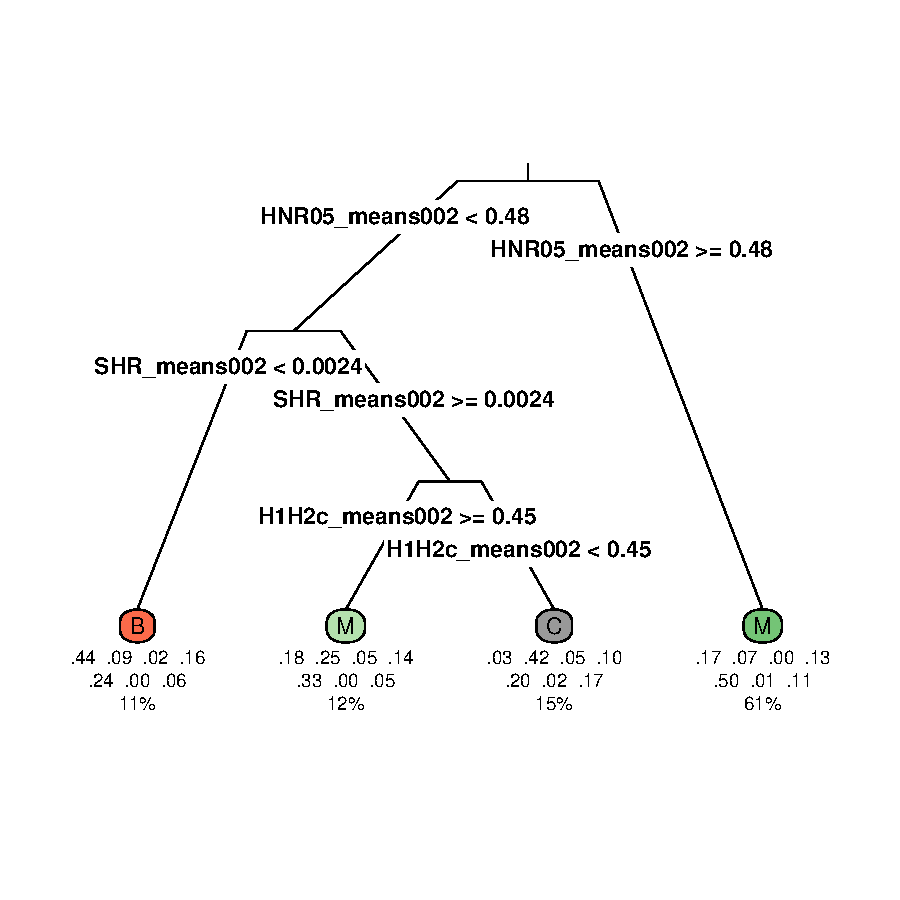
\includegraphics[width = 0.9\linewidth]{images/keating_tree.pdf}
    \caption{Classification tree of phonation categories from \citet{keatingCrosslanguageAcousticSpace2023}. Abbreviations used in this figure are: {HNR05_means002}: harmonics-to-noise ratio over the frequency range from 0 Hz to 500 Hz for the middle third of each vowel; {SHR_means002}: subharmonic-to-harmonic ratio for the middle third of each vowel; {H1H2c_means002}: H1* − H2* for the middle third of each vowel; B: breathy, M: modal, and C: creaky phonation categories.}
    \label{fig:keating_tree}
\end{figure}

In the analysis presented in this chapter, I will make use of bagging trees to assess the importance of the different 

% Description: This file contains the content of the chapter 3 of the dissertation. It is based on an article that me and Grant wrote.

%------------------------------------------------
\chapter{On using Residual H1* for voice quality research} \label{ch:residual_h1}
%------------------------------------------------
%------------------------------------------------
\section{Introduction} \label{sec:Intro}
%------------------------------------------------

Languages use voice quality distinctions to convey phonemic distinctions \citep{garellekPhoneticsVoice2019} and to convey paralinguistic information by ``indexing the biological, psychological, and social characteristics of the speaker" \citep{laverVoiceQualityIndexical1968,podesvaStanceWindowLanguageRace2016}. Voice quality contrasts have been studied extensively by examining their correlates in the acoustic signal \citep[e.g.,][]{espositoCrossLinguisticPatterns2020}, resulting in a large and complex literature on acoustic correlates of phonation differences \cite[see][]{garellekPhoneticsVoice2019}. 

One measure that is by far the most commonly applied is H1*$-$H2*, which measures the relative amplitudes of the first harmonic and second harmonic. As established by Fischer-Jorgensen, the relative strength of the fundamental is a correlated measure of breathy voice in contrast with modal voice \citet{fischer-jorgensenPhoneticAnalysisBreathy1968}. In order to normalize the amplitude of the fundamental and counteract some of the effects of high-pass filtering and differences in sound pressure in the signal, she proposed that you could subtract the amplitude of a higher harmonic, in this case, the second harmonic (H2), from the amplitude of the fundamental (H1). Since its introduction, H1*$-$H2* has been used in many studies to measure not only breathy voice but other voice quality contrasts as well \citep{garellekPhoneticsVoice2019,chaiH1H2Acoustic2022}.

Despite the large amount of evidence in support of H1*$-$H2*, it is not without its problems. At the fundamental level, it is not clear that H1*$-$H2* adequately measures the strength of the fundamental. \citet{sundbergObjectiveCharacterizationPhonation2022} found that H1 and H2 are affected differently by subglottal pressure, compromising some of the original reasoning behind the use of H1*$-$H2* from \citet{fischer-jorgensenPhoneticAnalysisBreathy1968}. Similarly, in a comprehensive overview of the main concerns with H1*$-$H2* as a phonation type measure, \citet{chaiH1H2Acoustic2022} found that in addition to the issues mentioned above, errors in measuring H1*$-$H2* are uncomfortably high. This is mainly due to the need to precisely measure two different harmonic amplitudes; when there are errors in calculating H1, this, in turn, leads to errors in calculating H2 \citep{arrasIntroductionErrorPropagation1998}. An example of this type of error propagation is that errors in measuring the fundamental frequency, which is especially common with non-modal phonation, are introduced into measuring harmonics because they are based on the fundamental. Despite algorithms correcting for vowel height, a common error that occurs is when a high fundamental frequency co-occurs with a low first formant \citep{chaiH1H2Acoustic2022}. This situation causes errors in tracking the fundamental frequency and the first formant. A final issue that can occur when measuring the harmonics is in contexts where the vowel is nasalized. \citet{simpsonFirstSecondHarmonics2012} shows that in these nasalized contexts, the first nasal pole (P0) can increase the amplitude of H2 and, when the fundamental frequency is high, H1 increases instead.

This collection of errors leads \citet{chaiH1H2Acoustic2022} to propose a new measure, residual H1*. This measure is calculated by first regressing H1 on energy and then subtracting the product of energy and the energy factor from H1. Chai and Garellek argue that this measure better reflects the initial purpose of using H1*$-$H2*. Furthermore, they find that residual H1*: (i) provides better differentiation between phonation types in !Xóõ; (ii) was more robust for measuring creak in Mandarin with respect to different utterance positions; and (iii) has a stronger relationship to the open quotient than H1*H2* based on a comparison using EEG data.

The contributions \citet{chaiH1H2Acoustic2022} make are very intriguing and have the potential to alter how spectral analyses of voice quality are performed. However, they are not convincing on their own. If residual H1* is to be widely adopted in linguistics, speech pathology, and other speech sciences, then it requires considerable evidence of its effectiveness in acoustic studies. This paper offers additional evidence for residual H1*'s effectiveness. 

Given the promising nature of this measure, we tested residual H1* with data from Santiago Laxopa Zapotec. Although \citet{chaiH1H2Acoustic2022} evaluated residual H1* for !Xóõ and Mandarin, both of which contain tone and voice quality, they do not factor tone into their analysis.\footnote{!Xóõ is most like Zapotec in that it has three phonologized phonation categories. It also has tone, which to our understanding is not restricted by phonation and which is not analyzed in \citet{chaiH1H2Acoustic2022}. The Mandarin case is less relevant as its phonation is prosodic and tonally linked.} This is where testing the effectiveness of residual H1* in Zapotec languages is beneficial. Zapotec languages are often described as laryngeally complex \citep{silvermanLaryngealComplexityOtomanguean1997,ariza-garciaPhonationTypesTones2018}. Laryngeal complexity is defined as a language that allows contrastive tone and contrastive voice quality that are unrestricted in their interactions. This laryngeal complexity between tone and phonation types presents a unique challenge for acoustic analysis and testing of the residual H1* measure. 

Other Zapotec languages have also been studied for voice quality research. For example, \citet{espositoVariationContrastivePhonation2010} found that in Santa Ana del Valle Zapotec there was a biological sex difference in which acoustic measures best capture the voice quality contrasts similar to observations from \citet{klattAnalysisSynthesisPerception1990}. \citet{arellanesarellanesDosGradosLaringizacion2010} found that the realization of laryngealization in a variety of San Pablo Güilá Zapotec is highly variable and depends on the position of laryngealization in the phrase. This was also found to be the case in Betaza Zapotec \citep{crowhurstInfluenceVowelLaryngealisation2016}. \citet{barzilaiContextdependentPhoneticEnhancement2021} found that tone and phrasal position also played a role in how voice quality is realized in San Pablo Macuiltianguis Zapotec. These studies show that Zapotec languages have much to contribute to our understanding of voice quality. 

We find that residual H1* can adequately capture differences in voice quality and is a more robust measure of voice quality than H1*$-$H2*, adding credence to the use of this measure instead of H1*$-$H2* in voice quality research. The remainder of this paper is organized as follows. Section~\ref{sec:SLZ} provides a brief overview of the Santiago Laxopa Zapotec language. Section~\ref{sec:Methods} describes the methods used in the data collection, data processing, and statistical modeling used in this study. Section~\ref{sec:Results} presents the results of the study. Section~\ref{sec:Conclusion} concludes the paper.

%----------------------------------------------------------------------------------------
\section{Santiago Laxopa Zapotec} \label{sec:SLZ}
%----------------------------------------------------------------------------------------
Santiago Laxopa Zapotec is a Northern Zapotec language of the Oto-Manguean language family \citep{adlerAcousticsPhonationTypes2016,adlerDerivationVerbInitiality2018,foleyForbiddenCliticClusters2018,foleyExtendingPersonCaseConstraint2020,sichelPronounsAttractionSierra2020,
sichelFeaturalLifeNominals2020,brinkerhoffDownstepSantiagoLaxopaMFM,brinkerhoffTonalPatternsTheir2022}. It is spoken by 981 people in the municipality of Santiago Laxopa, Ixtlán, Oaxaca, Mexico and a small number of other speakers from the diaspora in Mexico and the United States. 

Santiago Laxopa Zapotec exhibits a four-vowel inventory (that is, /i/, /e/, /a/, and /u/), which is further distinguished by a four-way contrast in voice quality. This variety is unique because it is a Northern Zapotec that has developed a breathy voice (/V̤/) in addition to the two types of laryngealization that characterize the rest of the Zapotec languages, namely checked and articulated. Checked vowels are defined as a modal vowel that ends with a period of creaky voice or a glottal closure (/VV̰/ or /Vˀ/ ). Rearticulated vowels are also defined as a modal vowel that also has a period of creakiness or glottal closure but aligned to the middle of a vowel (/VV̰V/ or /VˀV/). This makes an otherwise modal vowel appear as if it is interrupted by this laryngealization.\footnote{This is different from how rearticulated vowels are defined in other languages, where they are a modal vowel followed by an ``echo vowel" which may or may not have a glottal closure intervening between the modal and ``echo" vowel \citep[see][]{bairdPhoneticPhonologicalRealizations2011}. A fuller description of how these vowels are realized in one variety of Zapotec and the terms used are found in \citet{avelinoAcousticElectroglottographicAnalyses2010}.} This difference in laryngeal timing is one of the key differences between these phonations (see \cite{ariza-garciaPhonationTypesTones2018} for a detailed typological study of voice quality distinctions in Zapotec languages).

Santiago Laxopa Zapotec is also tonal with three level tones (H, M, and L) and two contours (MH and HL) appearing in nominals \citep{brinkerhoffTonalPatternsTheir2022}.\footnote{The tonal system of Santiago Laxopa Zapotec for verbs and other lexical categories is still being evaluated.} The language has a complex interaction between tone and phonation types. Every tone can appear with every phonation type, with two exceptions being that breathy voice cannot appear with the high tone and checked voice cannot appear with the rising contour tone. It is unclear whether these are accidental gaps or have a phonetic underpinning.

These interactions between voice quality and tone present a rich environment for testing the reliability of voice quality measures in laryngeally complex languages.

\section{Methods} \label{sec:Methods}
\subsection{Elicitation} \label{sec:Elicitation}

Ten native speakers of SLZ (five female; five male) participated in a wordlist elicitation. Elicitation was performed in the pueblo of Santiago Laxopa, Ixtlán, Oaxaca, Mexico during the summer of 2022 using the built-in microphone of a Zoom H4n handheld recorder (16-bit, 44.5 kHz). 

The wordlist consisted of 72 items repeated three times in isolation and the carrier sentence \textit{Shnia' X chonhe lhas} [ʃnːiaˀ X tʃone ɾas] ``I say X three times''. This sentence was chosen to minimize any effect of the phrasal position \citep[see][for a study about phrasal effects on voice quality in Zapotec]{crowhurstInfluenceVowelLaryngealisation2016}. Additionally, there are no co-articulatory effects on voice quality found with this frame and the items in the wordlist.  Between these 72 words, there were 11 words with breathy voice, 9 with rearticulated voice, 10 with checked voice, and 42 with modal. Thirteen of the 72 words were disyllabic and eight of the thirteen contained the same voice quality in each syllable. Of those 13 disyllabic word, only five contained different voice qualities in each of the syllables. This resulted in 85 different syllables.\footnote{There is ongoing debate about the status of strong syllables in Zapotec. The majority of evidence for the presence of stress comes from non-Northern Zapotec varieties \citep[e.g.,][]{chavez-peonPhoneticCuesStress2008,mockPitchAccentStress1988}. At this time, evidence for stress in Northern Zapotec remains to be seen.} 

The token selection for the wordlist was done in consultation with a native speaker. Similarly to \citet{barzilaiContextdependentPhoneticEnhancement2021}, we did not balance the tones with the different voice qualities. The frequency in which certain tones co-occur with certain voice qualities is uneven in the language, making it difficult to control for. The distribution of tones and voice quality across the 85 syllables used in this study are presented in Table~\ref{tab:distribution}. This imbalance was taken into account by including Tone as a fixed effect in our statistical models in Section~\ref{sec:StatisticalModeling}.

\begin{table}[!h]
  \centering
  \caption{Distribution of tone and voice quality in the wordlist}
  \label{tab:distribution}
    \begin{tabular}{llllll}
    \lsptoprule
    & High & Mid & Low & Rising & Falling\\
    \hline
    Modal & 14 & 9 & 15 & 2 & 10 \\
    Breathy & $-$ & $-$ & 11 & $-$ & 2 \\
    Checked & 1 & $-$ & 9 & $-$ & \\
    Rearticulated & 1 & $-$ & 4 & $-$ & 4 \\
    \lspbottomrule
    \end{tabular}
\end{table}


%----------------------------------------------------------------------------------------
\subsection{Data Processing} \label{sec:DataProcessing}
%----------------------------------------------------------------------------------------

Each vowel of the target words in the carrier sentence condition was labeled following \citet{garellekAcousticDiscriminabilityComplex2020} for where the vowel began and ended. Each vowel in the word list was annotated for speaker, word, vowel, tone, voice quality, and utterance number. This labeling was conducted for each vowel in the target word from the elicitation list of the carrier sentences.

These vowels were then extracted and fed into VoiceSauce for acoustic measurement \citep{shueVoiceSauceProgramVoice2011}. The formants were measured using Snack \citep{sjolanderSnackSoundToolkit2004}, while the fundamental frequency (\textit{f0}) was measured using the STRAIGHT algorithm \citep{kawaharaInstantaneousfrequencybasedPitchExtraction1998}. Spectral slope measures were corrected for formants and bandwidths \citep{hansonGlottalCharacteristicsFemale1997,iseliAgeSexVowel2007}. Each vowel was measured with ten equal time intervals, resulting in 22890 data points in total.

The data were cleaned of outliers following the same steps as taken by \citet{chaiH1H2Acoustic2022} in their study. The H1*, H1*–H2*, and \textit{f0} values were z-scored by speaker to reduce the variation between the speakers and provide a way to directly compare the different measures on the same scale. Data points with an absolute z-score value greater than 3 were considered outliers and excluded from the analyses. Within each vowel category, we calculated the Mahalanobis distance in the F1-F2 panel. Each data point with a Mahalanobis distance greater than 6 was considered an outlier and excluded from the analysis. Using the Mahalanobis distance allows us to compare the data points to the mean of the F1-F2 panel for each vowel category. The larger the Mahalanobis distance is the more deviant the data point is from the mean which in turn means that the data point was improperly tracked. This is comparable to what was done in \citet{seyfarthPlosiveVoicingAcoustics2018,chaiCheckedSyllablesChecked2022,garellekPhoneticsWhiteHmong2021}.

Time points whose \textit{f}0, F1, or F2 values were outliers were also excluded from H1* and H1*$-$H2* analyzes because H1* and H1*$-$H2* are calculated based on \textit{f0}, F1, and F2. Energy was excluded if it had a zero value and then logarithmically transformed to normalize its right-skewed distribution. Afterward, the resulting logarithmically transformed data was z-scored, and any data point with a z-score greater than 3 was excluded. This outlier removal resulted in 1918 datapoints being removed. 

After removing the outliers, we calculated residual H1* for the remaining data points following \citet{chaiH1H2Acoustic2022}. First, a linear mixed effects model was generated with the z-scored H1* as the response variable and the z-scored energy as the fixed effect. The uncorrelated interaction of the z-scored energy by speaker was treated as random. The energy factor resulting from this linear mixed-effects model was extracted. Finally, the z-scored H1* had the product of the z-scored energy and the energy factor subtracted from it, giving us the residual H1* measure.

The measures were then orthogonally coded according to their position in the vowel (first, middle, and third) and for tone (H, M, L, R, F) for statistical modeling.  

%----------------------------------------------------------------------------------------
\subsection{Statistical modeling} \label{sec:StatisticalModeling}
%----------------------------------------------------------------------------------------

Two linear mixed-effects regression models were fitted, one for the normalized H1*$-$H2* and residual H1*. Each model had the tone and the interaction between voice quality and position in the vowel as fixed effects. Vowel and interaction between the speaker, the word, and the repetition were treated as random intercepts.\footnote{ $Measure \sim  Phonation*Position + Tone + (1|Speaker:Word:Repetition) + (1|Vowel)$}

The tone and the interaction between voice quality and position in the vowel were selected as fixed effects for several reasons. The first is that five unique tones appeared in the data and it is well established that tone interacts with voice quality in different ways (see \cite{espositoCrossLinguisticPatterns2020} and \cite{garellekPhoneticsVoice2019} for discussion). By treating tone as a fixed effect in our model, we can account for these interactions. The interaction between voice quality and position in the vowel as a fixed effect was included to account for the temporal differences between the two different laryngealizations, checked and rearticulated vowels. Checked vowels in Zapotec languages have a glottal occlusion or a short period of creaky voice located at the right edge of the vowel. This is in contrast to rearticulated vowels, where there is a glottal occlusion or creaky voice in the middle of the vowel. Because this difference between checked and rearticulated vowels is temporal in nature, we can account for this difference through the interaction of voice quality and position in the vowel.\footnote{Tone and voice quality are closely linked. By including only the positional interaction with voice quality, we can avoid collinear interactions that appear when we try to include tone in the interaction.}

The interaction between speaker, word, and repetition was treated as a random intercept because this allows us to consider that each speaker said each word on the elicitation list three times. This intercept accounts for not only the intra-speaker variability, but also the inter-speaker variability during each time the word was uttered. Treating a vowel as a random intercept allows us to capture the fact that each voice quality occurred with different vowels during elicitation.

Additional statistical modeling was performed with two generalized additive mixed models (GAMM) using the \texttt{mgcv} package in R \citep{woodGeneralizedAdditiveModels2017}. The GAMMs were fitted to account for any non-linear effects that may be present in the data. In each case the response variable was the same as in the linear mixed-effects models with voice quality as a fixed effect. Splines where used to model the non-linear effects of position and position by phonation. Speaker and word were treated as random intercepts.
%----------------------------------------------------------------------------------------
\section{Results} \label{sec:Results}
%----------------------------------------------------------------------------------------

In interpreting the results, there are certain expectations about how these measures should capture the voice quality contrasts. As discussed in \citet{garellekPhoneticsVoice2019}, it is expected that breathy vowels should have a higher spectral slope than modal vowels across the two measures in keeping with observations about breathy vowels in other languages. Because both checked and rearticulated vowels make use of creaky voice, they should have a lower spectral slope than modal vowels. Additionally, because there is a temporal distinction between checked and rearticulated with where the creakiness appears, this should also be captured in the two measures. 

%----------------------------------------------------------------------------------------
\subsection{H1*$-$H2*} \label{sec:H1H2}
%----------------------------------------------------------------------------------------

Figure~\ref{fig:FIG1} shows the mean H1*$-$H2* values for each voice quality at each of the ten vowel intervals. We see that the breathy, checked, and rearticulated values are lower than the modal values at each of the first nine intervals. In the final intervals, breathy and rearticulated are essentially equal to the modal value. In contrast, checked's value remains lower than the modal's value throughout the entire vowel. This measure does not match the expectations discussed above.

\begin{figure}[htbp]
  \centering
  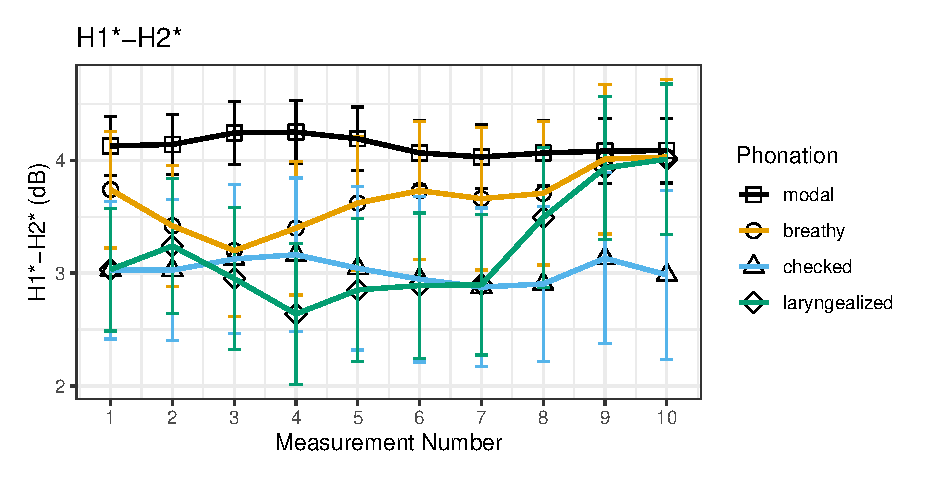
\includegraphics[width = 0.75\textwidth]{images/Figure1.eps}
  \caption{\label{fig:FIG1}{H1*$-$H2* across the duration of the vowel. Points represent the mean of each measure across the ten intervals. The error bars around each point represent a 95\% confidence interval. A line was plotted over each to show how the acoustic measure functions across the ten intervals.}}
\end{figure}

%----------------------------------------------------------------------------------------
\subsection{Residual H1*} \label{sec:ResidH1}
%----------------------------------------------------------------------------------------

Figure~\ref{fig:FIG2} shows the mean residual H1* values for each voice quality at each of the ten vowel intervals. In contrast to Figure~\ref{fig:FIG1}, we see that breathy has a higher residual H1* measure than modal throughout the duration of the vowel, which is consistent with other observations for breathy voice \citep{fischer-jorgensenPhoneticAnalysisBreathy1968}. Checked and rearticulated both have lower values than the modal at each of the 10 intervals. In addition, it shows that the checked voice has a lower residual H1 * value than the rearticulated voice at intervals 8 through 10. The rearticulated voice has a lower residual H1 * value than the checked voice at intervals 1 through 7, showing the temporal distinction between these two voice qualities. This measure complies with the expectations discussed above. 

\begin{figure}[htbp]
  \centering
  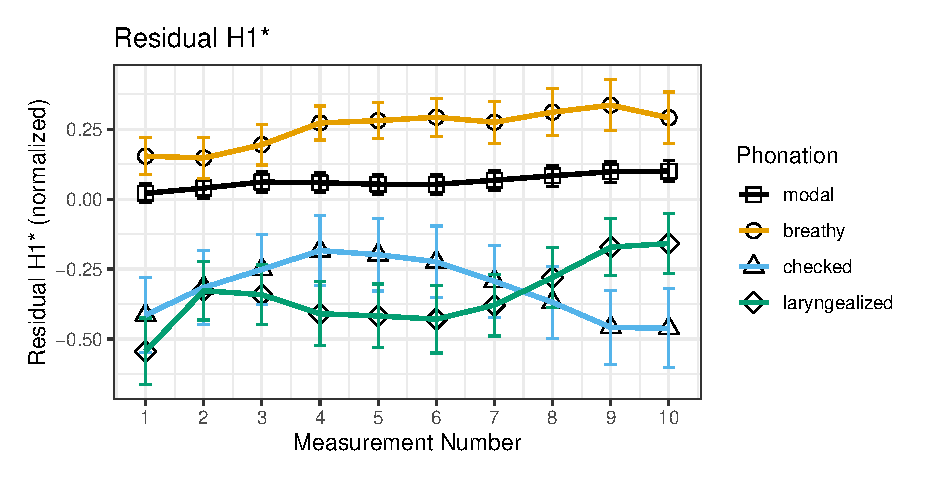
\includegraphics[width = 0.75\textwidth]{images/Figure2.eps}
  \caption{\label{fig:FIG2}{Residual H1* across the duration of the vowel. Points represent the mean of each measure across the ten intervals. The error bars around each point represent a 95\% confidence interval. A line was plotted over each to show how the acoustic measure functions across the ten intervals.}}
\end{figure}


%----------------------------------------------------------------------------------------
\subsection{Model Comparison} \label{sec:Comparison}
%----------------------------------------------------------------------------------------

To assess the robustness of the models, we compared the residual H1* linear mixed-effects model to the H1*$-$H2* linear mixed-effects model. This was done using two methods: direct comparison of the outputs of the two models in the same way as \citet{chaiH1H2Acoustic2022} and the Akaike Information Criterion (AIC). 

Table~\ref{tab:CGComparison} compares the linear mixed effects models for H1*$-$H2* and residual H1*. In comparing these models, we find that the residual H1* model performed better than the H1*$-$H2* model in distinguishing voice quality contrasts in Santiago Laxopa Zapotec. This is supported by the larger absolute value of the coefficient estimate, the lower standard error, and the higher t-value of the residual H1* to distinguish breathy, checked, and rearticulated vowels from modal vowels.

\begin{table}[!h]
  \centering
  \caption{Model comparison between H1*$–$H2* and Residual H1* in distinguishing Santiago Laxopa Zapotec voice quality.}
  \label{tab:CGComparison}
  % \begin{ruledtabular}
    \begin{tabular}{lllllll}
      \lsptoprule
    Voice Quality Contrast & Model & \textit{$\beta$ } & Std. Error & \textit{t}-value & \textit{p}-value  &     \\
    \hline
      Breathy vs Modal &  H1*$-$H2* & 0.04631 & 0.03806  & 1.21680 & 0.22372 & \\
      & Res. H1* & 0.23625 & 0.02866 & 8.24177   & \textless 0.001   & *** \\
      Checked vs Modal & H1*$-$H2* & -0.11880 & 0.03476 & -3.41793  & \textless 0.001 & *** \\
      & Res. H1* & -0.40099 & 0.02621 & -15.30098 & \textless 0.001 & *** \\
      Rearticulated vs Modal & H1*-H2 & -0.09175 & 0.04588 & -1.99968 & 0.04560 & *  \\
     & Res. H1* & -0.44162 & 0.03450 & -12.80027 & \textless 0.001 & *** \\
     \lspbottomrule
    \end{tabular}
  % \end{ruledtabular}
\end{table}

Table~\ref{tab:Comparison} shows the results of the AIC comparison between the H1*$-$H2* and residual H1* models. The residual H1* model had a lower AIC than the H1*$-$H2* model, indicating that the residual H1* model is a better fit for the data than the H1*$-$H2* model. Although AIC comparison is usually performed on nested models, it is still a useful tool for comparing non-nested models \citep{burnhamMultimodelInferenceUnderstanding2004,burnhamAICModelSelection2011,burnhamModelSelectionMultimodel2004}.

\begin{table}[!h]
  \centering
  \caption{AIC for the H1*$-$H2* and residual H1* models.}
  \label{tab:Comparison}
  % \begin{ruledtabular}
  \begin{tabular}{lll}
    \lsptoprule
    Model  & AIC & $\Delta$ AIC\\
    \hline
    H1*$-$H2* model & 43443.33 & 11182.76 \\
    Residual H1* model & 32260.57 & 0 \\
    \lspbottomrule
  \end{tabular}
  % \end{ruledtabular}
\end{table}

%---------------------------------------------------------
\subsection{GAMM analysis and model comparisons} \label{sec:GAMM}
%---------------------------------------------------------

The GAMM analysis shows that there are non-linear effects present in the data. This was expected because of the dynamic nature of the voice quality in SLZ. Figures~\ref{fig:GAMM_h1h2} and \ref{fig:GAMM_residh1} show the GAMM smooths and difference plots for H1*$-$H2* and residual H1*, respectively. The difference plots in each figure show the difference between the smooths for each voice quality compared to modal.

Do to the nature of GAMM analyses, it is important to visually inspect the results to see how well the model fits the data. The model that best fits the data is the one that shows the clearest distinction between the different voice qualities.

In Figure~\ref{fig:GAMM_h1h2}, we see that the different voice qualities are very difficult to observe clearly. In the top left panel, the smooth functions of the GAMM analysis are shown. In it we see that modal and breathy voice occupy the same space. However, checked and rearticulated voice are more separated from modal, with both appearing lower in the graph. The difference plot in the top right show that for breathy vs. modal there was no significant difference between the two voice qualities in term of H1*$-$H2*. In the bottom left, the difference plot shows that the differences we observe between checked and modal voice is significant across the entire duration of the vowel. The difference plot in the bottom right shows that there is a significant difference between rearticulated and modal voice in the first two thirds of the vowel, but not in the final third of the vowel.

\begin{figure}[!ht]
  \centering
  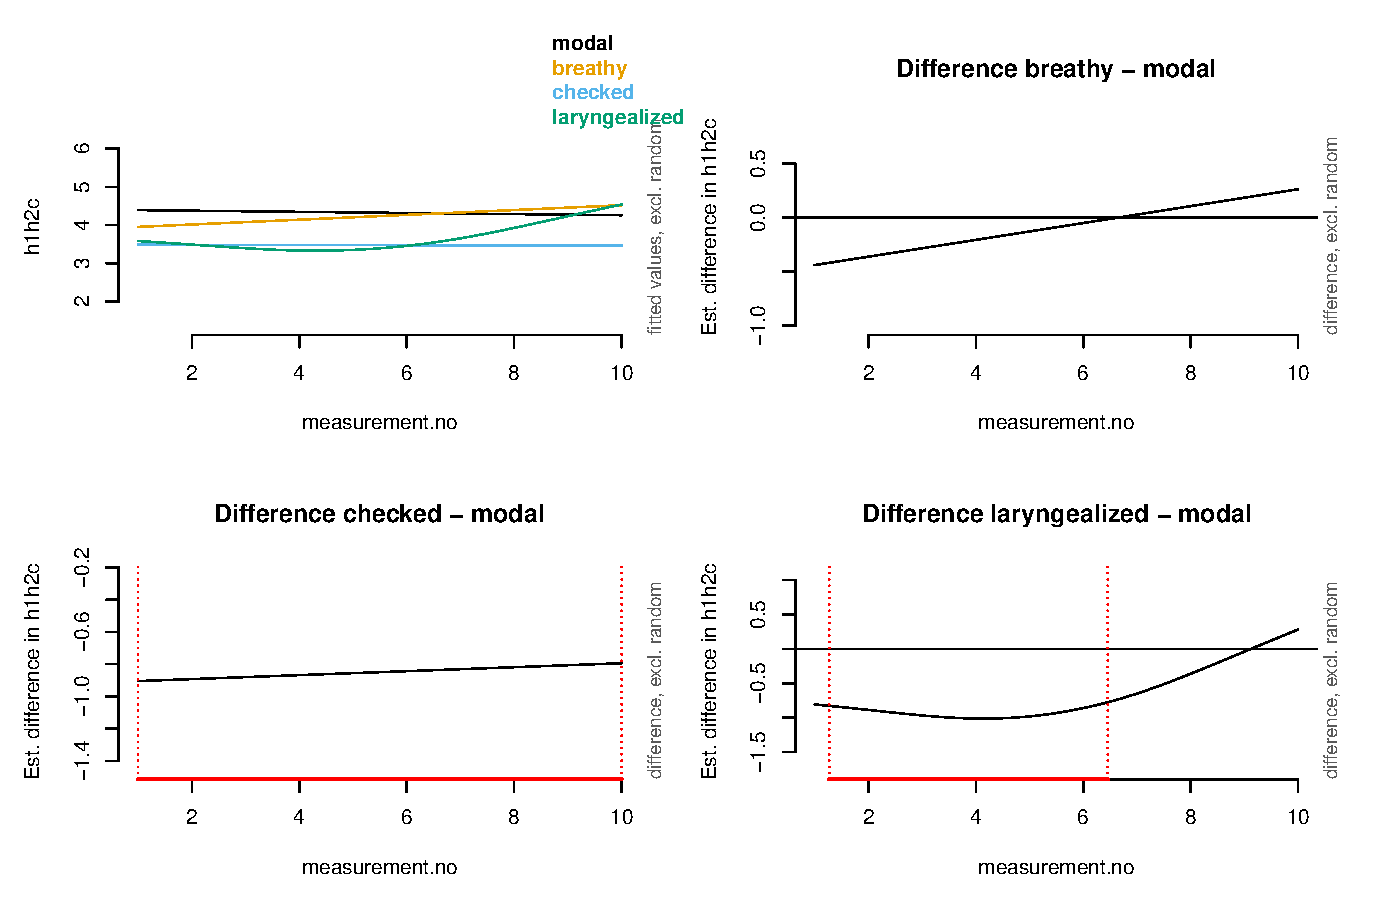
\includegraphics[width = \textwidth]{images/h1h2_gamm.eps}
  \caption{GAMM smooths and difference plots for H1*$-$H2* across the duration of the vowel.}
  \label{fig:GAMM_h1h2}
\end{figure}


The residual H1* shows a clearer distinction between the different voice qualities than H1*$-$H2*. This is especially clear in the difference plots, where the difference between breathy and modal is much more pronounced in the residual H1* than in H1*$-$H2*.

\begin{figure}[!ht]
  \centering
  \includegraphics[width = \textwidth]{images/residh1_gamm.eps}
  \caption{GAMM smooths and difference plots for residual H1* across the duration of the vowel.}
  \label{fig:GAMM_residh1}
\end{figure}
%% Before bibliography:

\section{Conclusion} \label{sec:Conclusion}

In conclusion, we find that residual H1* is a more robust measure of voice quality than H1*$-$H2* in Santiago Laxopa Zapotec. This is supported by the results of the linear mixed-effects models, which show that residual H1* is better at distinguishing breathy, checked, and rearticulated vowels from modal vowels. This is further supported by the AIC comparison, which shows that the residual H1* model is a better fit for the data than the H1*$-$H2* model. These results lend credence to the claims of \citet{chaiH1H2Acoustic2022} and support using residual H1* instead of H1*$-$H2* in voice quality research, especially in laryngeally complex languages.

However, the results neither suggest nor support the notion that residual H1* should be the sole measure used to determine phonation quality. Instead, we suggest that residual H1* should be included as one of the measures that researchers should consult during their acoustic studies. 
\include{contents/5.previous}
\chapter{Conclusion}

%--------------------------------------------------------------------------
%  Bibliography
%--------------------------------------------------------------------------
% LTeX: enabled=false
%%-----------------------------------------
%% Bibliography 
%%-----------------------------------------
%%% Not that I use amsrefs
% \clearpage
\phantomsection
	%\bibliography{Thesis.bib}
\begin{bibdiv}
	\addchaptertocentry{}{Bibliography}% Add bib title to toc
\begin{biblist}

%Put your bib entires here.

\end{biblist}
\end{bibdiv}
% N.B. by default I use raw amsrefs. If you prefer to let amsrefs load .bib file, use the following instead:
%\bibliography{yourbibfile}

\appendix
%Appendix chapter
\chapter{Wordlist}

\begin{longtable}{lllll}
\lsptoprule
 Lexeme & Eng. Gloss & Sp. Gloss & Phonation   & Tone   \\
\midrule
 \textit{xa'ag}  & sheriff, police    & \textit{topíl} & R & L \\
 \textit{xmanh}  & week  & \textit{semana}    & M & HL \\
 \textit{xche}   & dinner & \textit{cena} & M & H \\
 \textit{yu'u}   & house & \textit{casa}  & R & HL    \\
 \textit{rmedzw} & remedy    & \textit{remedio}   & M & H \\
 \textit{yu'}    & earth & \textit{tierra}    & C & L \\
 \textit{za'a}   & corncob   & \textit{elote} & R & HL \\
 \textit{behl}   & snake & \textit{vibora}    & B & L \\
 \textit{tsil}   & in the morning    & \textit{en la mañana} & M & HL \\
 \textit{bel}    & fish & \textit{pez} & M & HL \\
 \textit{bzine'} & rat; mouse & \textit{ratón} & MC & LL \\
 \textit{bedzjw} & turkey    & \textit{guajolote} & M & H \\
 \textit{rbej}   & pea   & \textit{chícharo}  & M & L \\
 \textit{behb}   & trash & \textit{basura}    & B & L \\
 \textit{bene'}  & person & \textit{persona} & MC & MH \\
 \textit{yich}   & paper & \textit{papel} & M & L \\
 \textit{dam}    & owl & \textit{tecolote/buho} & M & H \\
 \textit{blull}  & frog; toad & \textit{sapo; rana} & M & L \\
 \textit{yag}    & measure of corn   & \textit{almúd} & M & L \\
 \textit{bgah}   & necklace; bracelet & \textit{collar} & B & L \\
 \textit{behlhe'} & meat & \textit{carne} & BC & LL \\
 \textit{lni}    & party & \textit{fiesta} & M & L \\
 \textit{jid}    & chicken & \textit{gallina} & M & MH \\
 \textit{bdze'}  & ant & \textit{hormiga} & C & L \\
 \textit{yichbahlh} & midnight & \textit{madrugada/medianoche}  & B & LHL    \\
 \textit{chi'im (bi'a ser)} & honey & \textit{miel de abeja} & R & H \\
 \textit{ya'a}   & market & \textit{mercado} & R & L \\
 \textit{llume}  & basket & \textit{canasta} & MM & MH \\
 \textit{xwe}    & lunch & \textit{comida} & M & L \\
 \textit{xsil}   & breakfast & \textit{almuerzo} & M & L \\
 \textit{yell}   & village & \textit{pueblo} & M & HL \\
 \textit{behche'} & wasp's nest & \textit{panal/nido de avispas} & BC & LL \\
 \textit{yej}    & flower & \textit{flor} & M & L \\
 \textit{shchag} & noise & \textit{ruido} & M & HL \\
 \textit{deh}    & ash & \textit{ceniza} & B & L \\
 \textit{bxhillu'} & badger; coati & \textit{tejón} & MC & HL \\
 \textit{kampanh} & bell & \textit{campana} & MM & MHL    \\
 \textit{cha'}   & cooking pot & \textit{cazuela} & C & L \\
 \textit{lhe'ej} & fence; corral & \textit{cerca; jaripeo} & R & HL \\
 \textit{chib}   & goat & \textit{chivo} & M & HL \\
 \textit{xhidw}  & cat & \textit{gato} & MW & MH \\
 \textit{bo'}    & coal & \textit{carbón} & C & L \\
 \textit{bsuh}   & adobe & \textit{adobe} & B & HL \\
 \textit{ze'e}   & wall & \textit{pared} & RR & HL \\
 \textit{pantlon} & pants & \textit{pantalones} & MM & MHL \\
 \textit{sukr}   & sugar & \textit{azucar} & M & H \\
 \textit{gwanhax} & garlic & \textit{ajo} & MM & LHL \\
 \textit{iz}     & year & \textit{año} & M & L \\
 \textit{bxhidw} & kiss & \textit{beso} & M & M \\
 \textit{yitw}   & pumpkin & \textit{calabaza} & M & HL \\
 \textit{beht}   & skunk & \textit{zorrillo} & B & L \\
 \textit{yah}    & iron; rifle & \textit{fierro; rifle} & B & L \\
 \textit{pyine}  & bird & \textit{pájaro} & MM & MM \\
 \textit{yet}    & tortilla & \textit{tortilla} & M & L \\
 \textit{lok}    & angry & \textit{enojado} & M & L \\
 \textit{biu'walh} & full moon & \textit{luna llena} & M & H \\
 \textit{zix}    & sweet & \textit{dulce} & M & H \\
 \textit{shlkan/kandadw} & lock & \textit{candado} & MM & MH \\
 \textit{player} & t-shirt & \textit{playera} & MM & MH \\
 \textit{botey}  & bottle  & \textit{botella} & MM & MH \\
 \textit{duh}    & rope; cord & \textit{mecate; cuerda} & B & L \\
 \textit{da'abep}    & reed & \textit{capisallo} & RM & L \\
 \textit{yi'inh} & chili pepper & \textit{chile} & R & L \\
 \textit{blli'in} & beast of burden; mule & \textit{bestia; mulo} & R & HL \\
 \textit{zahg} & cold & \textit{frío} & B & L \\
 \textit{zah}    & bean & \textit{frijol} & B & L \\
 \textit{xkalh}  & mayor & \textit{alcalde} & M & L \\
 \textit{xtilh}  & white & \textit{blanco}  & M & HL \\
 \textit{chich}  & white & \textit{blanco} & M & H      \\
 \textit{libr}   & book & \textit{libro} & M & H \\
 \textit{yag}    & tree; wood & \textit{árbol} & M & L \\
\lspbottomrule
\end{longtable}


\end{document}
